\documentclass[11pt]{article}
% Load Packages
%%%%%%%%%%%%%%%%%=
\usepackage[margin=1in]{geometry}
\geometry{letterpaper}
\addtolength{\oddsidemargin}{-0.3in}
\addtolength{\topmargin}{-0.3in}
\addtolength{\textheight}{0.3in}
\addtolength{\evensidemargin}{-0.3in}
\addtolength{\textwidth}{0.6in}
\usepackage{lineno}
\usepackage{enumitem}
\usepackage{multicol}
\usepackage{fixltx2e}
\usepackage{amsmath,amsfonts,amsthm,amssymb}
\usepackage{graphicx}
\usepackage{tikz,pgfplots}
\usepackage[noend]{algpseudocode}
\usepackage{algorithm,algorithmicx}
\usepackage{url}
\usepackage{color}
\usepackage{varioref}
\usepackage{mathrsfs}
\usepackage[sort&compress,colon,square,numbers]{natbib}
\usepackage{subcaption}
\usepackage[final,authormarkup=none]{changes}
\usepackage{framed}
\usepackage{setspace}
\usepackage{verbatim}
\usepackage{multicol}
\usepackage{dblfloatfix}
\usepackage{wrapfig}
\usepackage{float}
\usepackage{amssymb}
\usepackage{verbatim}
\usepackage{booktabs,colortbl, array}
\usepackage{pgfplotstable,tabularx}
\usepackage{tikz}
\usepackage{pifont}% http://ctan.org/pkg/pifont
\usepackage{caption}
\usepackage{enumitem}% http://ctan.org/pkg/enumitem
\captionsetup[figure]{font=small}
\captionsetup[table]{font=small}

%% Set bibliography style
%%%%%%%%%%%%%%%%%%%%%%%%%%%%%%%%%==%%%%%s
%~~

\renewcommand{\labelenumi}{\Arabic{enumi}}

%% Declare Colors
%%%%%%%%%%%%%%%%%%%%%%%%%%%%%%%%%%%%%==%

\definecolor{darktangerine}{rgb}{1.0, 0.77, 0.07}
\definecolor{aogr}{rgb}{0.0, 0.5, 0.0}

%% Set Up Checks/Xs

\newcommand{\cmark}{\ding{51}}%
\newcommand{\xmark}{\ding{55}}%
\newcommand{\boldq}{\textbf{?}}

\newcommand{\greencheck}{\textcolor{aogr}\cmark}
\newcommand{\ocheck}{\textcolor{darktangerine}\cmark}
\newcommand{\yellowq}{\textcolor{darktangerine}\boldq}
\newcommand{\redx}{\textcolor{red}\xmark}

%% Set up Tables
%%%%%%%%%%%%%%%%%%%%%%%%%%%%%%%%%%%%%===%
\definecolor{tableheadcolor}{gray}{0.92}
% Following is taken from Werner: http://tex.stackexchange.com/a/33761/3061
% and modified for my needs
%
% Command \topline consists of a (slightly modified)
% \toprule followed by a \heavyrule rule of colour tableheadcolor
% (hence, 2 separate rules)
\newcommand{\topline}{ %
        \arrayrulecolor{MSBlue}\specialrule{0.1em}{\abovetopsep}{0pt}%
        \arrayrulecolor{tableheadcolor}\specialrule{\belowrulesep}{0pt}{0pt}%
        \arrayrulecolor{MSBlue}}
% Command \midline consists of 3 rules (top colour tableheadcolor, middle colour black, bottom colour white)
\newcommand{\midtopline}{ %
        \arrayrulecolor{tableheadcolor}\specialrule{\aboverulesep}{0pt}{0pt}%
        \arrayrulecolor{MSBlue}\specialrule{\lightrulewidth}{0pt}{0pt}%
        \arrayrulecolor{white}\specialrule{\belowrulesep}{0pt}{0pt}%
        \arrayrulecolor{MSBlue}}
% Command \bottomline consists of 2 rules (top colour
\newcommand{\bottomline}{ %
        \arrayrulecolor{white}\specialrule{\aboverulesep}{0pt}{0pt}%
        \arrayrulecolor{MSBlue} %
        \specialrule{\heavyrulewidth}{0pt}{\belowbottomsep}}%


\newcommand{\midheader}[2]{%
        \midrule\topmidheader{#1}{#2}}
\newcommand\topmidheader[2]{\multicolumn{#1}{c}{\textsc{#2}}\\%
                \addlinespace[0.5ex]}

\pgfplotstableset{normal/.style ={%
        header=true,
        string type,
        font=\addfontfeature{Numbers={Monospaced}}\small,
    	column type={p{.092\textwidth}},
        every odd row/.style={
            before row=
        },
        every head row/.style={
            before row={\topline\rowcolor{tableheadcolor}},
            after row={\midtopline}
        },
        every last row/.style={
            after row=\bottomline
        },
        col sep=&,
        row sep=\midrule
    }
}
% Setup Tikz Plots
%%%%%%%%%%%%%%%%%==
\tikzset{
    flowbox/.style={
        rectangle, rounded corners, minimum width=2cm, minimum height=1cm,text centered, draw=black
    },
    stdarrow/.style={->,>=latex, line width=1.5pt}
}
\pgfplotsset{compat=newest}

% Define Some Math Operators
%%%%%%%%%%%%%%%%%%%%%===
\labelformat{equation}{\textup{(#1)}}
\DeclareMathOperator*{\rank}{rank}
\DeclareMathOperator*{\trace}{trace}
\DeclareMathOperator*{\range}{range}
\DeclareMathOperator*{\spn}{span}
\DeclareMathOperator*{\acos}{acos}
\DeclareMathOperator*{\argmax}{arg\,max}
\DeclareMathOperator*{\argmin}{arg\,min}
\DeclareMathOperator*{\Discriminability}{\textit{Discriminability}}
\DeclareMathOperator*{\iid}{\overset{iid}{\sim}}

% Define custom column widths
%%%%%%%%%%%%%%%%%%%%%%%%%%%%%=
\setlength{\columnsep}{1cm}
\setlist[enumerate, 1]{label=\textbf{\alph*.}}
\usepackage{array}
\newcolumntype{L}{>{\raggedright\arraybackslash}m{3.55cm}}
\newcolumntype{Q}{>{\raggedright\arraybackslash}m{3.35cm}}

% TODOs 
%%%%%===
\newcommand{\todo}[1]{{\color{red}{\it TODO: #1}}}
\newcommand{\greg}[1]{{\color{cyan}{\it greg: #1}}}
\newcommand{\jovo}[1]{{\color{purple}{\it jovo: #1}}}

% Shorthand
%%%%%%%%%===
\newcommand{\sic}[0]{{\textsc{SIC}}}
\newcommand{\ndmg}[0]{{\textsc{NDMG}}}
\newcommand{\ndmgd}[0]{{\textsc{NDMG-d}}}
\newcommand{\ndmgf}[0]{{\textsc{NDMG-f}}}

\usepackage{neurodata}

\usepackage{enumitem}

\title{
A Low-Resource Pipeline to Democratize Multi-Modal Connectome Estimation and Analysis
% A High-Throughput Pipeline Identifies Robust Connectomes But Troublesome Variability
}


\begin{document}

\maketitle
\noindent\parbox{0.9\textwidth}{
\normalsize\color{lgray} Gregory~Kiar$^*$, Eric~W.~Bridgeford$^*$,  William~R.~Gray~Roncal$^*$, 
Consortium for Reliability and Reproducibility (CoRR), 
Vikram~Chandrashekhar, Disa~Mhembere,  Sephira~Ryman,  Xi-Nian~Zuo,  Daniel S.~Margulies, R. Cameron Craddock, Carey E.~Priebe,
Rex~Jung, Vince~D.~Calhoun, 
Brian Caffo, Randal~Burns, Michael P.~Milham,  
Joshua~T.~Vogelstein$^\dagger$
\\%$^1$
%Johns Hopkins University, University of New Mexico, %$^2$
%Child Mind Institute, \& University of Chinese Academy of Sciences
%,\& Research Center for Lifespan Development of Mind and Brain (CLIMB), Institute of Psychology, Chinese Academy of Sciences
}
\thispagestyle{empty}
\medskip
\vspace{10pt}


\noindent
\textbf{%
Human brain imaging using magnetic resonance imaging (MRI) has recently undergone received widespread attention.  These data potentially hold the key to understanding both normal and abnormal brain function.  Connectomics, the study of connections in the brain, has recently been implicated as a potential route to such discoveries.  However, MRI based connectomics is a resource intensive practice.  MRI machines cost millions of dollars, and  studies cost thousands of dollars per individual.  Moreover, state of the art analysis routines require both extensive domain expertise, as well as considerable computational power and capabilities.  These challenges are in stark contrast to the recent globalization of brain sciences, with the advent of various national and international brain initiatives.  We therefore built a low-resource functional and diffusion MRI pipeline to estimate and analyze human connectome data.  Running the pipeline, without any manual intervention, on approximately 6,000 open access brain scans, and making all data derivatives open, results in the largest open access human connectome repository in the world.  Our open source pipeline, and resulting data derivatives, therefore democratizes connectomics, welcoming participation from researchers previously unable to contribute to our community.
% Modern scientific discovery depends on collecting large heterogeneous datasets with many sources of variability, and applying domain-specific pipelines from which one can draw  insight or clinical utility. For example, macroscale connectomics studies require complex pipelines to process raw functional or diffusion data and estimate connectomes. Individual studies tend to customize pipelines to their needs, raising concerns about their reproducibility,  and adding to a longer list of factors that may differ across studies (including sampling, experimental design, and data acquisition protocols), resulting in failures to replicate. Mitigating these issues requires multi-study datasets and the development of pipelines that can be applied across them. We developed NeuroData's MRI to Graphs (\ndmg) pipeline using several functional and diffusion studies, including the Consortium for Reliability and Reproducibility, to estimate connectomes. Without any manual intervention or parameter tuning, \ndmg~ran on 25 different studies ($\approx$ 6,000 scans) from 15 sites,  with each scan resulting in a biologically plausible connectome (as assessed by multiple quality assurance metrics at each processing stage). For each study, the connectomes from \ndmg~are more similar within than across individuals, indicating that \ndmg~is preserving biological variability. Moreover, the connectomes exhibit near perfect consistency for certain connectional properties across every scan, individual, study, site, and modality; these include stronger ipsilateral than contralateral connections and stronger homotopic than heterotopic connections.  Yet, the magnitude of the differences varied across individuals and studies---much more so when pooling data across sites, even after controlling for study, site, and basic demographic variables (i.e., age, sex, and ethnicity). This indicates that other experimental variables (possibly those not measured or reported) are contributing to this variability, which if not accounted for can limit the value of aggregate datasets, as well as expectations regarding the accuracy of findings and likelihood of replication. We, therefore, provide a set of principles to guide the development of pipelines capable of pooling data across studies while maintaining biological variability and minimizing measurement error. This open science approach provides us with an opportunity to understand and eventually mitigate spurious results for both past and future studies.
}
%Modern scientific discovery depends on collecting large heterogeneous datasets with many sources of variability, and applying domain-specific pipelines from which one can draw  insight or clinical utility. For example, macroscale connectomics studies require complex pipelines to process raw functional or diffusion data and estimate connectomes. Individual studies tend to customize pipelines to their needs, raising concerns about their reproducibility,  and adding to a longer list of factors that may differ across studies (including sampling, experimental design, and data acquisition protocols), resulting in failures to replicate. Mitigating these issues requires multi-study datasets and the development of pipelines that can be applied across them. We developed NeuroData's MRI to Graphs (NDMG) pipeline using several functional and diffusion studies, including the Consortium for Reliability and Reproducibility, to estimate connectomes. Without any manual intervention or parameter tuning, NDMG ran on 25 different studies (~6,000 scans) from 15 sites,  with each scan resulting in a biologically plausible connectome (as assessed by multiple quality assurance metrics at each processing stage). For each study, the connectomes from NDMG are more similar within than across individuals, indicating that NDMG is preserving biological variability. Moreover, the connectomes exhibit near perfect consistency for certain connectional properties across every scan, individual, study, site, and modality; these include stronger ipsilateral than contralateral connections and stronger homotopic than heterotopic connections. Yet, the magnitude of the differences varied across individuals and studies - much more so when pooling data across sites, even after controlling for study, site, and basic demographic variables (i.e., age, sex, and ethnicity). This indicates that other experimental variables (possibly those not measured or reported) are contributing to this variability, which if not accounted for can limit the value of aggregate datasets, as well as expectations regarding the accuracy of findings and likelihood of replication. We, therefore, provide a set of principles to guide the development of pipelines capable of pooling data across studies while maintaining biological variability and minimizing measurement error. This open science approach provides us with an opportunity to understand and eventually mitigate spurious results for both past and future studies.

\begin{multicols}{2}


% @AK: "if you mean failures in surface reconstruction by FreeSurfer, I didn't mention in the Mindboggle article that 1/3 of our EMBARC subjects' surface reconstructions were deemed unfit for further analysis, but:
% http://journals.plos.org/ploscompbiol/article?id=10.1371/journal.pcbi.1005350
% Figure 2 shows gyral crown clipping.
% And: " For 16 cortical regions in the 40 subjects, we measured scan-rescan reliability of cortical thickness measures, and we compared thickness measures with published estimates based on manual delineations of MR images of living brains [115]. Forty percent of FreeSurfer estimates for the 640 labels were in the published ranges of values ...  (as mentioned above, Klauschen observed that FreeSurfer underestimates gray matter and overestimates white matter [78]). " 

% @GK: we can fix how we do tensor estimation and stuff in native space with this: https://www.mitpressjournals.org/doi/abs/10.1162/NETN_a_00035


\section{Introduction}

Human brain imaging potentially holds the key to unlocking mysteries that psychologists, psychiatrics, and neurologists have been struggling with for centuries.  Magnetic Resonance Imaging (MRI) has become a vital tool both in basic brain science, as well as neurology~\cite{}.  The true potential of these data, however, remains unmet.  For example, while much effort has been devoted to clinical brain imaging~\cite{}, our community is yet to provide a brain imaging based biomarker for any psychiatric condition~\cite{}.  Moreover, our community is currently facing a bit of a reproducability crisis, partially due to different researchers using different analysis techniques, and partially because sample sizes are too small~\cite{}.  Both of these issues could be mitigated by expanding the community of individuals studying brain science, to bring in fresh and complementary perspectives of dedicated individuals.  And excitement for this possibility is global: with many countries recently announcing national and international brain initiatives, we now have an opportunity to collectively tackle some of these challenges.  Importantly, all countries can be motivated by the challenges associated with human brain imaging, as data from the World Health Organization suggests that mental and behavioral disorders are largest burden of disease, worldwide~\cite{Whiteford13, Vigo16}.


Collecting these data, however, is quite expensive.  A new MRI machine costs millions of dollars.  Moreover, maintaining a machine requires a full time physicits, and each imaging session  costs thousands of US dollars.  Such obstancles limit the acquisition of data to relatively rich countries, institutions, and researchers.  It is not just data acquisition that is expensive, data analysis is also costly.  Recently proposed methods for individual stages of MRI brain processing can each take over a day per scan, and memory exceeding the standard alotment on laptops.  Thus, even if data were available, and individuals acquired the highly specialized knowledge to process the data, doing so is often financially out of reach.  Finally, there is an emerging global community of data scientists, partially due to the availability of massive online open courses, such as Coursera's Data Science Specialization, which has trained over 5 million individuals world wide.  These data scientists could contribute to solving the problems connectomics faced, if they had access to data in formats that they could understand and parse, rather than raw data or derivatives in MRI specific formats. 




% that provide the necessary data~\cite{corr}. But no existing pipeline can successfully estimate and meaningfully process every scan in this dataset---including both functional and diffusion data---while also quantifying the magnitude and source of variability amongst them. 
% We, therefore, established several principles and metrics to guide the development of pipelines.  
We developed an approach, ``Neuro Data MRI to Graphs'' (\ndmg), that 
can run on various quality datasets without parameter change or manual intervention. It does not seek to obtain the best possible estimates of connectivity from a given dataset; such a goal would require dataset specific tuning, and likely more computationally expensive algorithms. It does however provides extensive quality assurace at each data processing stage, and outputs organized and in formats familiar to data scientists.  The final output for each individual is a set of connectomes (functional or structural map of connectivity) at 24 different spatial resolutions.



We validated our pipeline by running \ndmg~on the entirety of data from the Consortium of Reliability and Reproducibility (CoRR).  The CoRR data  consists of about 30 different studies from nearly 20 different institutions around the world, spanning the Americas, Europe, and Asia. The CoRR data collection efforts were not harmonized, and all data (regardless of quality) were shared.  Thus, these data are well-suited to test the robustness of any pipeline.  We also ran \ndmg~on several additional open access dataset with complementary acquisition parameters. In total, we ran \ndmg~on 11 dMRI  studies comprising 3,227 individuals with 4,347 scans, and 18 fMRI  studies comprising 714 individuals with 1,646 scans---yielding a total of nearly  $150,000$ estimated connectomes---all of which are publicly available from \url{http://m2g.io}. 

\ndmg~ran to completion, estimating connectomes at multiple scales, on every scan, thus providing strong evidence that it can be used widely on other future datasets, including data from low-resource communities leveraging older MRI technology.  Moreover, the resulting connectomes constitute  the largest open database of connectomes to date~\cite{brown2016connected}.  Although these connectomes were estimated using computationally expedient algorithms, they look like connectomes derived from state of the art processing pipelines, requiring days to process each scan, rather than an hour. We therefore expect this pipeline and dataset to democratize connectomics, both by providing a pipeline that brain scientists can apply ``out of the box'' on their data, and providing a large and fully processed dataset for subsequent analysis. 
% and one of the largest mega-analyses (inference across studies) of multi-modal connectomics data to date~\cite{varoquaux2013learning, vidaurre2017discovering}. 



% These connectomes provided the data that led us to develop statistical connectomics methods to quantify various connectome properties, such as the relative probability of ipsilateral vs.~contralateral connections and homotopic vs.~heterotopic connections. While these properties have been previously noted in single studies~\cite{Stark2008,Zuo2010,Gee2011}, this work demonstrates that aspects of these properties are preserved both across individuals and studies upon optimizing and harmonizing the pipeline. Nonetheless, within session, site, study, and demographic cohorts, substantial variability remained in the \emph{magnitude} of these properties. 
% Moreover, we observed a considerably higher degree of variability across sites, studies, and demographic cohorts. In part, this variability may be due to legitimate biological heterogeneity that could not be accounted for using the limited phenotyping available. However, a substantial portion of that variability is likely reflective of experimental and/or measurement error.
% This variability can partially explain recent failures of replicability in neuroimaging~\cite{Button2013}, as well as the lack of clinically useful neuroimaging based biomarkers~\cite{APA12}. This work therefore motivates significant further efforts in measurement and/or analysis to mitigate ``batch effects’’ in neuroimaging. 
% Other disciplines with similar findings have resolved these issues by revolutionizing their measurement strategy (for example, genomics moved away from microarrays because sequencing can be significantly more reliable than microarray measurements~\cite{SEQCMAQC-III_Consortium2014-ij})---though only after all efforts to remediate existing methods failed. For imaging, more comprehensively phenotyped individuals, and more coordinated data acquisition protocols, can be a first step towards studies generating sufficiently accurate and reliable inferences and clinical biomarkers.

%%%%%%%%
% % tbd post submission: add AMI for ndmg.
\begin{table*}
    \centering
    \caption{\textbf{Comparing M3R Processing Pipelines.}
\ndmg~is designed  with both algorithmic and implementation principles in mind.  This table compares existing pipelines along these  principles, demonstrating that for each, \ndmg~ performs at least as well as the current state of the art. A  \greencheck~is given for pipelines that satisfy the respective desiderata, a \ocheck~for pipelines that partially satisfy the respective desiderata, and a \redx~is given for pipelines that do not satisfy the respective desiderata.   \ref{app:pipes} provides more details.}
\label{tab:pipelines}
    \pgfplotstabletypeset[
        header=true,
        string type,
        font=\addfontfeature{Numbers={Monospaced}}\small,
        columns/pipe/.style={column name={pipeline}, column type={p{.1\textwidth}}},
        columns/acc/.style={column name={\rotatebox{60}{accurate}}, column type={p{.05\textwidth}}},
        columns/rel/.style={column name={\rotatebox{60}{reliable}}, column type={p{.05\textwidth}}},
        columns/rob/.style={column name={\rotatebox{60}{robust}}, column type={p{.05\textwidth}}},
        columns/exp/.style={column name={\rotatebox{60}{expedient}}, column type={p{.05\textwidth}}},
        columns/scale/.style={column name={\rotatebox{60}{scalable}}, column type={p{.05\textwidth}}},
        columns/port/.style={column name={\rotatebox{60}{portable}}, column type={p{.05\textwidth}}},
        columns/tk/.style={column name={\rotatebox{60}{turn-key}}, column type={p{.05\textwidth}}},
        columns/open/.style={column name={\rotatebox{60}{open}}, column type={p{.05\textwidth}}},
        columns/dwi/.style={column name={\rotatebox{60}{dMRI}}, column type={p{.05\textwidth}}},
        columns/fmri/.style={column name={\rotatebox{60}{fMRI}}, column type={p{.05\textwidth}}},
        columns/end2end/.style={column name={\rotatebox{60}{raw-to-graph}}, column type={p{.06\textwidth}}},
        every head row/.style={
            before row={
                \topline
                \rowcolor{tableheadcolor}
                & \multicolumn{4}{c}{Statistical Principles} & \multicolumn{4}{c}{Computational Principles} & \multicolumn{3}{c}{Connectome Principles}\\
                \rowcolor{tableheadcolor}
            },
            after row={\midtopline}
        },
        every odd row/.style={
            before row={\rowcolor{vlgray}}
        },
        every last row/.style={
            after row=\bottomline
        },
        col sep=&,
        row sep=\\
    ]{pipe & acc & rel & rob & exp & scale & port & tk & open & dwi & fmri & end2end \\
    
\includegraphics[width=.025\textwidth]{neurodata_small}\ndmg & \ocheck & \greencheck & \greencheck & \greencheck & \greencheck & \greencheck & \greencheck & \greencheck & \greencheck & \greencheck  & \greencheck \\
    HCP \cite{glasser2013} & \ocheck & \greencheck & \greencheck & \greencheck & \redx & \redx & \greencheck & \greencheck & \greencheck & \greencheck & \redx \\
    PANDA\cite{Cui2013} & \ocheck & \greencheck & \greencheck & \greencheck & \ocheck & \ocheck & \ocheck & \greencheck & \greencheck & \redx &  \greencheck \\
    CMTK\cite{Daducci2012} & \ocheck & \greencheck & \greencheck & \greencheck & \ocheck & \redx & \redx & \ocheck & \greencheck & \redx &  \greencheck  \\
    CPAC\cite{cpac}  & \ocheck & \greencheck & \greencheck & \greencheck & \greencheck & \greencheck & \greencheck & \greencheck  &  \redx & \greencheck & \redx \\
    fmriprep\cite{esteban_oscar_2017_1044752} & \ocheck & \greencheck & \greencheck & \redx & \greencheck & \greencheck & \greencheck & \greencheck & \redx & \greencheck & \redx  \\
    NIAK\cite{bellec2011} & \ocheck & \greencheck & \greencheck & \greencheck & \ocheck & \ocheck & \redx & \ocheck & \redx & \greencheck & \redx  \\
    }
% \caption*{}
\end{table*}

%%%%%%%%



\section{Results}


% \subsection{Individual-Level Analysis}

\begin{figure*}[t!]
	\centering
	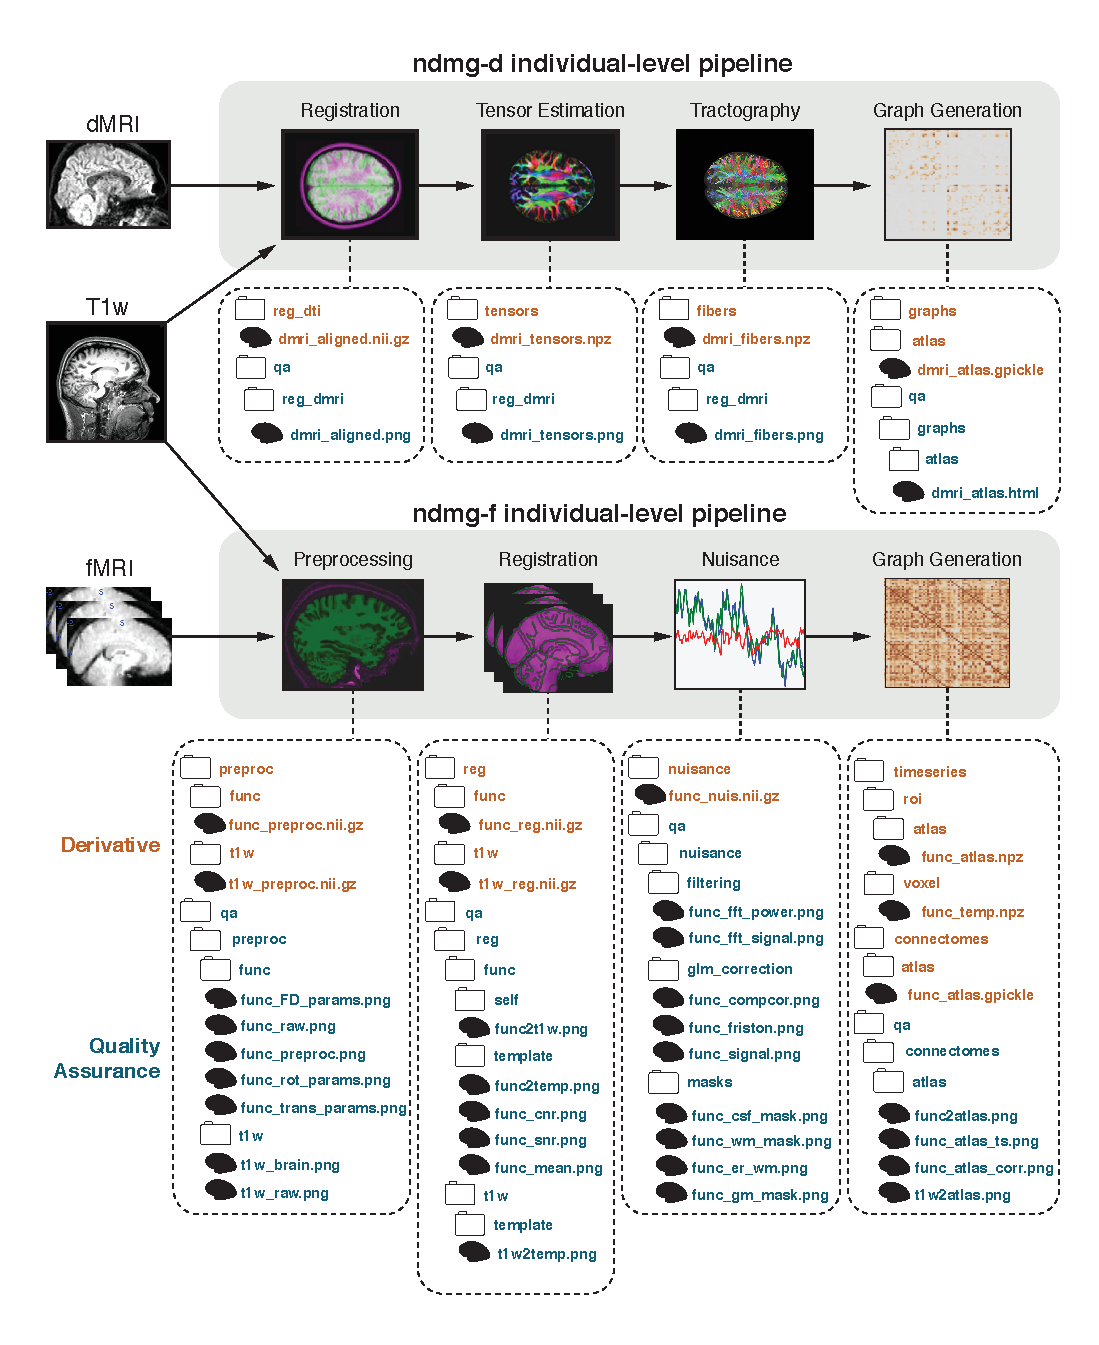
\includegraphics[width=0.9\textwidth]{./figs/ndmg_pipeline.pdf}
    \caption{\textbf{Individual Level Pipeline}
  The individual-level  \ndmg~pipeline has two sub-pipelines:  (1) \ndmgd~transforms raw dMRI data into sparse structural connectomes, and (2) \ndmgf~transforms raw fMRI data into dense functional connectomes.  Each sub-pipeline consists of four key steps, and each step generates both data derivatives and quality assurance figures to enable both qualitative assessments and quantitative comparisons (see~\ref{app:dpipe} and~\ref{app:fpipe} for details).  
%  as seen in the top. \ndmgd~consists of four main steps: registration, tensor estimation, tractography, and graph generation. Simiarly, the subject-level of the \ndmgf~pipeline transforms raw functional MRI data into structural connectomes, as seen in the bottom. \ndmgf~consists of four main steps: preprocessing, registration, nuisance-correction, and graph generation.
%  At each stage, \ndmg~produces both data derivatives and quality assurance figures of the derivative, as illustrated.
}
	\label{fig:ndmgpipeline}
\end{figure*}

% \clearpage
%%%%%%%
%\begin{table*}
    \centering
    \caption{\textbf{\ndmg~pipeline robustness and reliability.}
We ran \ndmg~on over 20 different studies, including both fMRI and dMRI data, spanning multiple different scanners, acquisition parameters, and population demographics. Nonetheless, for both fMRI and dMRI data, across all datasets with multiple measurements, \ndmg~always achieved $>0.8$ discriminability, and \ndmgd's discriminability was typically $>0.98$ on the dMRI data. MM computes discriminability using multi-modal data from both the dMRI and fMRI connectomes. $D$=discriminability. Scanners are G (GE), P (Phillips), or S (Siemens).	
}
    \label{tab:data}
    \pgfplotstabletypeset[
    	header=true,
        string type,
        font=\addfontfeature{Numbers={Monospaced}}\small,
        columns/dset/.style={column name=Study, column type={p{.115\textwidth}}},
        columns/sca/.style={column name=Scanner, column type={p{.064\textwidth}}},
        columns/age/.style={column name={Age$\pm$1 std}, column type={p{.106\textwidth}}},
        columns/male/.style={column name=$\%$ Male, column type={p{.06\textwidth}}},
        columns/subjs/.style={column name=Indiv., column type={p{.055\textwidth}}},
        columns/ses/.style={column name=Ses., column type={p{.04\textwidth}}},
        columns/totd/.style={column name=\#Scans, column type={p{.049\textwidth}}},
        columns/trtd/.style={column name=$D$, column type={p{.048\textwidth}}},
        columns/totf/.style={column name=\#Scans, column type={p{.06\textwidth}}},
        columns/trtf/.style={column name=$D$, column type={p{.048\textwidth}}},
        columns/totm/.style={column name=\#Scans, column type={p{.049\textwidth}}},
        columns/trtm/.style={column name=$D$, column type={p{.048\textwidth}}},
        every head row/.style={
            before row={
            	\topline
                \rowcolor{tableheadcolor}
            },
            after row={\midtopline}
        },
        every odd row/.style={
        	before row={\rowcolor{vlgray}}
        },
        every row no 25/.style={
            before row={\topline\rowcolor{tableheadcolor}}
        },
        every last row/.style={
            before row={\rowcolor{tableheadcolor}},
            after row=\bottomline
        },  
        col sep=&,
        row sep=\\
    ]{dset & subjs & ses & totd & trtd \\
    HNU1    & 30   & 10 & 300  & 0.993  \\
    BNU1    & 57   & 2  & 114  & 0.984 \\
    SWU4    & 235  & 2  & 454  & 0.884 \\
    BNU3    & 48   & 1  & 47   & NA \\
    Kirby21 & 21   & 2  & 42   & 1.0 \\
    NKI1    & 24   & 2  & 40   & 0.984 \\
    Temp114 & 114  & 1  & 114  & NA  \\
    NKI-ENH & 198  & 1  & 198  & NA  \\
    Temp255 & 255  & 1  & 253  & NA \\
    PING    & 932  & 1-5& 1486 & NA \\
    MRN1313 & 1313 & 1  & 1299 & NA\\
    Pooled dMRI & 3227 & & 4347& 0.979 \\
    }
\end{table*}

\begin{table*}
    \centering
    \caption{\textbf{\ndmg~pipeline robustness and reliability.}
We ran \ndmg~on over 20 different studies, including both fMRI and dMRI data, spanning multiple different scanners, acquisition parameters, and population demographics. Nonetheless, for both fMRI and dMRI data, across all datasets with multiple measurements, \ndmg~always achieved $>0.8$ discriminability, and \ndmgd's discriminability was typically $>0.98$ on the dMRI data. MM computes discriminability using multi-modal data from both the dMRI and fMRI connectomes. $D$=discriminability. Scanners are G (GE), P (Phillips), or S (Siemens).	
}
    \label{tab:data}
    \pgfplotstabletypeset[
    	header=true,
        string type,
        font=\addfontfeature{Numbers={Monospaced}}\small,
        columns/dset/.style={column name=Study, column type={p{.115\textwidth}}},
        columns/sca/.style={column name=Scanner, column type={p{.064\textwidth}}},
        columns/age/.style={column name={Age$\pm$1 std}, column type={p{.106\textwidth}}},
        columns/male/.style={column name=$\%$ Male, column type={p{.06\textwidth}}},
        columns/subjs/.style={column name=Indiv., column type={p{.055\textwidth}}},
        columns/ses/.style={column name=Ses., column type={p{.04\textwidth}}},
        columns/totd/.style={column name=\#Scans, column type={p{.049\textwidth}}},
        columns/trtd/.style={column name=$D$, column type={p{.048\textwidth}}},
        columns/totf/.style={column name=\#Scans, column type={p{.049\textwidth}}},
        columns/trtf/.style={column name=$D$, column type={p{.048\textwidth}}},
        columns/totm/.style={column name=\#Scans, column type={p{.06\textwidth}}},
        columns/trtm/.style={column name=$D$, column type={p{.048\textwidth}}},
        every head row/.style={
            before row={
            	\topline
                \rowcolor{tableheadcolor}
            },
            after row={\midtopline}
        },
        every odd row/.style={
        	before row={\rowcolor{vlgray}}
        },
        every row no 25/.style={
            before row={\topline\rowcolor{tableheadcolor}}
        },
        every last row/.style={
            before row={\rowcolor{tableheadcolor}},
            after row=\bottomline
        },  
        col sep=&,
        row sep=\\
    ]{dset & subjs & ses & totf & trtf \\
    HNU1     &  30  & 10 & 300 & 0.956  \\
    BNU1     & 57   & 2  & 108 & 0.906  \\
    SWU4     & 235  & 2  & 466 & 0.891  \\
    BNU3     & 48   & 1  & 47  & NA  \\
    IPCAS6   & 2    & 9  & 18  & 0.994 \\
    IPCAS8   & 13   & 2  & 26  & 0.958  \\
    SWU1     & 20   & 3  & 60  & 0.935  \\
    IPCAS5   & 22   & 2  & 44  & 0.819 \\
    SWU3     & 23   & 2  & 46  & 0.986 \\
    XHCUMS   & 23   & 5  & 115 & 0.823 \\
    UWM      & 25   & 2  & 50  & 0.849 \\
    NYU1     & 25   & 3  & 75  & 0.931 \\
    SWU2     & 27   & 2  & 54  & 0.874 \\
    IPCAS1   & 30   & 2  & 60  & 0.893 \\
    IPCAS2   & 34   & 2  & 68  & 0.868 \\
    IBATRT   & 36   & 2  & 50  & 0.974 \\
    MRN1     & 52   & 2  & 90  & 0.859 \\
    BNU2     & 61   & 2  & 121 & 0.863 \\
    }
\end{table*}
%%%%%%%

\subsection{Individual-Level Analysis}

% In the individual-level analysis, in each session, multiple imaging a given  individual  undergoes some number of sessions, during which multiple different modalities can be collected.
The input to \ndmg~for a given individual is  the collection of scans and some metadata for each scan, including a structural scan, % (T1w/MPRAGE), 
and either, or both of, (1) a diffusion scan, including the diffusion parameters files,  and (2) a functional scan, including the slice acquisition sequence.
The individual-level of \ndmg~analysis leverages existing open source tools, including
the fMRI Software Library (FSL) ~\cite{fsl1, fsl2, fsl3}, Dipy~\cite{dipy}, the MNI152 atlas~\cite{mni152}, and a variety of parcellations defined in the MNI152 space~\cite{desikan, aal, jhu, harvardoxford, talairach, slab907, slab1068, pvt, glasser} (see \ref{app:parcels} for details about included parcellations). 
% @reb: vince says: [hey, we have a number of ICA parcellation schemes, the way we like to use them is to run spatially constrained ICA on new data using these as priors...if you want to do something with this let me know, possible collaboration going forward? ;-) ] let's get them in our set?
All algorithms requiring hyper-parameter selection were initially set to the suggested parameters for each tool, and tuned to improve the accuracy, reliability, expediency, and robustness of the results.
The output of each processing stage includes data derivatives and QA figures to enable individualized accuracy assessments.
% The QA figures at many stages include cross-sectional images at different depths in the three canonical planes (sagittal, coronal, and axial) of images or overlays. 
Figure~\ref{fig:ndmgpipeline} provides a schematic of the individual-level analysis, and Appendix  
\ref{app:pipe} provides further details, as well as some example quality assurance figures.

The \ndmgd~pipeline consists of: (1) registration, (2) tensor estimation, (3) tractography, and (4) graph generation. It was optimized on the Kirby21 dataset, and then applied to the remaning 10 datasets.
Individual-level analysis in \ndmgd~takes approximately $1.5$ hours to complete using 1~CPU core and 12~GB of RAM at 1 mm$^3$ resolution.
The individual-level analysis was run on 11 studies, including 3,227 individuals and 4,347 scans, using 24 parcellations,  resulting in 104,328 functional connectomes.

The \ndmgf~pipeline consists of: (1) preprocessing, (2) registration, (3) nuisance correction, and (4) graph generation.
The \ndmgf~pipeline was constructed starting with the optimal processing pipeline identified in Wang et. al~\cite{discriminability} using CPAC~\cite{cpac}. 
Individual-level analysis in \ndmgf~takes approximately 20~minutes to complete using 1~CPU core and 3~GB of RAM at 2 mm$^3$resolution.
The individual-level analysis was run on 714 individuals with 1,646 scans from 18 studies, generating connectomes across each of the 24 parcellations in \ndmgd, and resulting in 39,504 total connectomes.

All data derivatives, including the nearly 150,000 estimated connectomes, as well as quality assurance figures, are available from \url{https://m2g.io}.  We hope these data will provide a useful resource for others studying connectomics, especially those in data science fields such as graph theory and social network analysis, that lack the subject matter expertise to estimate connectomes, but have much to add to our community in terms of downstream analysis.


\subsection{Multi-Group-Level Analysis}

% We ran \ndmg~on the 11 diffusion and 18 functional studies listed in  Table~\ref{tab:data}.
% For each, \ndmg~group-level analysis computes and plots group-level graph summary and reliability statistics. 

% \subsection{Multi-Study Analysis}

We focus our group level analysis on the resulting connectomes, as this pipeline is designed to be a connectome estimation and analysis pipeline.  Specifically, for each connectome, we compute eight different metrics, many of them multivariate (see Appendix for details).  For each study, we then compute the average over individuals.  Figure~\ref{fig:multisite} accumulates the results over all the studies.  It is readily apparent that \ndmg~successfully estimates connectomes from each study, even though the data quality, scanner parameters, and population demographics differ quite widely.  This is a testament to the robustness of \ndmg.  

% top panel shows a variety of uni- and multi-variate statistics of the average diffusion connectome from each of the studies enumerated in Table~\ref{tab:data} with diffusion data using the Desikan parcellation. The bottom panel shows the same statistics computed on the average functional connectome from each of the studies enumerated in Table~\ref{tab:data} with functional data using the Desikan parcellation. In both the diffusion and functional connectomes, each dataset largely appears to have similar trends across each of the statistics shown.

\begin{figure*}[t!]
    \centering
    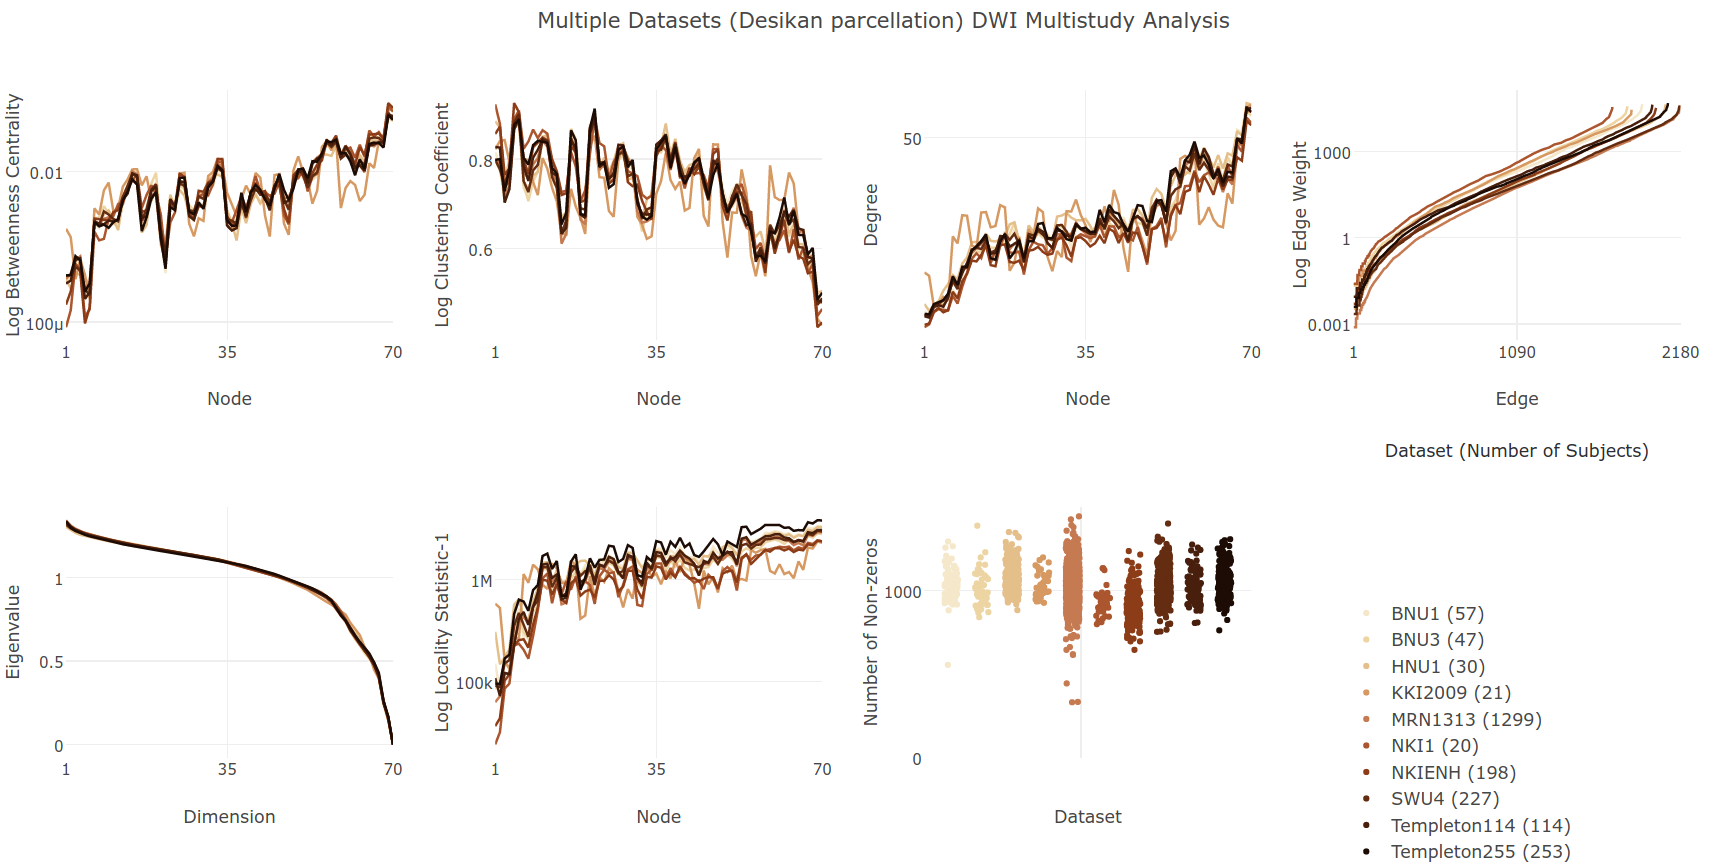
\includegraphics[width=\textwidth]{./figs/fig_dwi_multisite.png}
    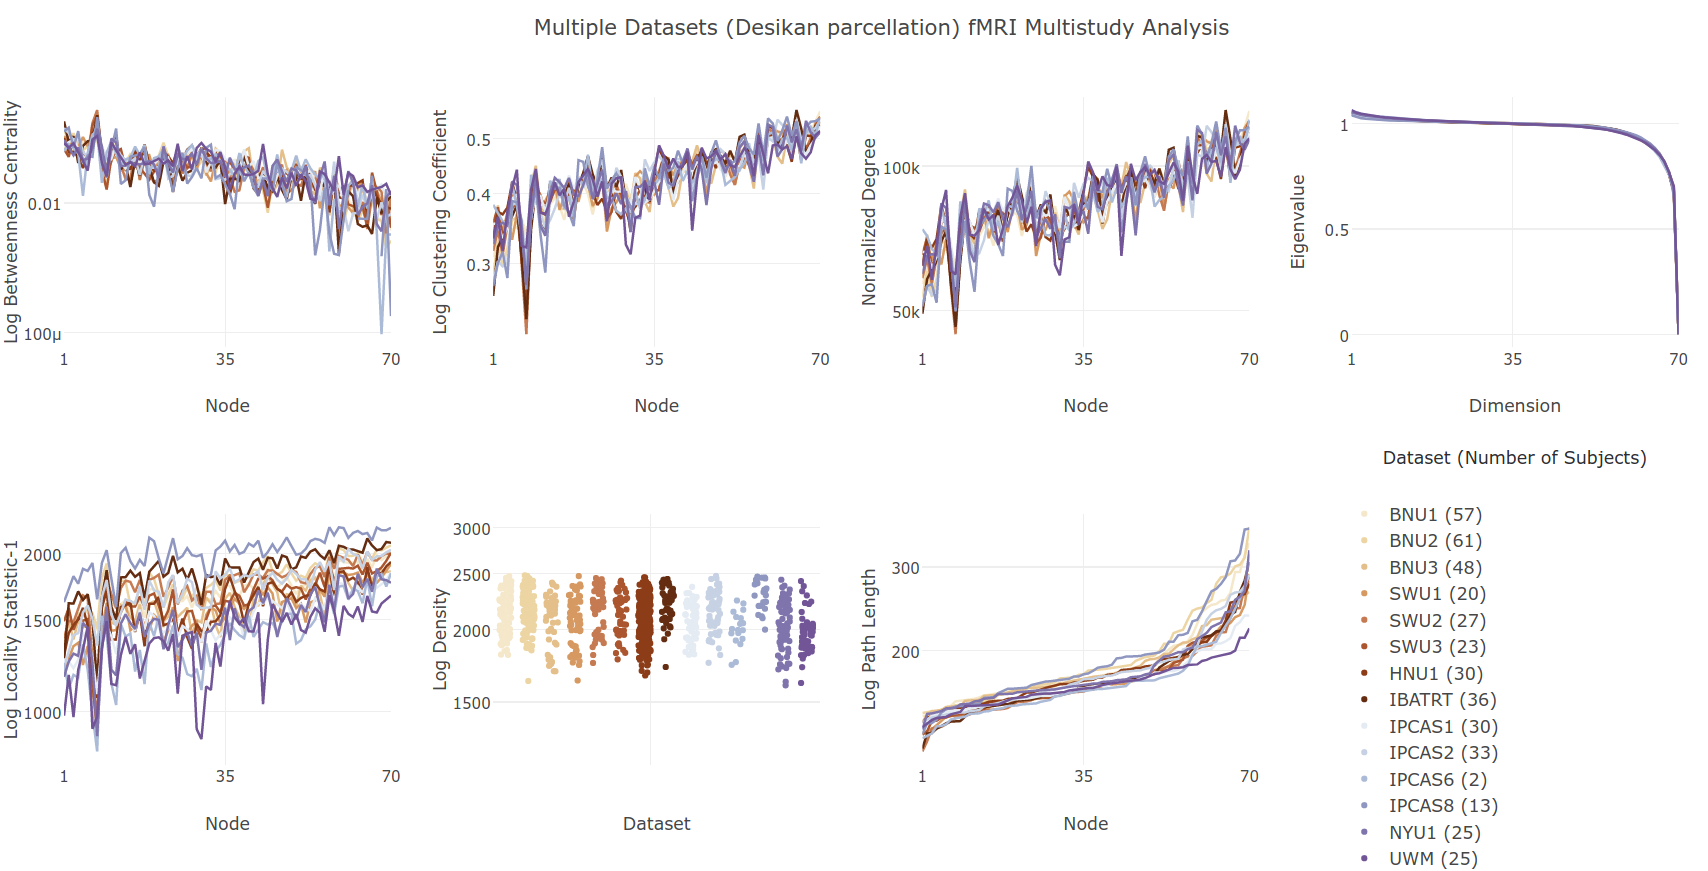
\includegraphics[width=\textwidth]{./figs/fig_fmri_multisite.png}
    \caption{
    \textbf{Multi-Study Connectome Analysis}.
    Average connectomes from ten (seventeen) diffusion (functional) studies processed with \ndmgd~are qualitatively compared by way of their summary statistics on the Desikan parcellation in the top (bottom).
    The Desikan atlas used in \ndmg~has been modified to include two additional regions, one per hemisphere, which fills in a hole in the parcellation near the corpus callosum.
    The nodes in this plot have been sorted such that the degree sequence of the left hemisphere (Desikan nodes 1-35) of the BNU1 dataset is monotonically non-decreasing, and that corresponding left-right nodes are next to one another.
    Each line shows the average for each statistic over all individuals within a study.
    % On  the bottom, we repeat the same analysis on the functional connectomes from seventeen different studies. Like the statistics computed in for the diffusion connectomes, t
    The statistics are  qualitatively similar across studies. 
    % This suggests that claims made or analyses
    % performed on a given scale may not hold when applied to another scale. Again, we see that parcellation choice has an impact on the implications of a study. Information on the graph statistics computed can be found in \ref{app:graphstats}.
    }
    \label{fig:multisite}
\end{figure*}


% \clearpage
\subsection{Comparison to Resource Intensive Pipelines}


\section{Discussion}


% The goal of any scientific investigation is not to characterize the observed sample data’s variance, but rather, to make inferences about the general population on the basis of those data.  
% Variability of sample demographics, data acquisition details (for example, number of repetitions for fMRI, number of directions for dMRI), analysis methods, measurement error, questionable research practices, or statistical errors can each contribute to limitations in generalizing to populations in psychology~\cite{Button2013} and neuroimaging~\cite{Costafreda2009}.
% Our principles for pipeline development enabled a rigorous high-throughput analysis of multi-study, multi-site, and multi-connectome data to identify and quantify different sources of variability.

% While perhaps seemingly at odds, the results from Figures~\ref{fig:siem} and~\ref{fig:batch} are complementary.  Specifically, Figure~\ref{fig:siem} demonstrates that essentially all connectomes share a particular property: stronger connections in one set of edges than another. On the other hand, Figure~\ref{fig:batch} demonstrates that although some sets of edges tend to be larger than others, the {magnitude} of the differences is highly variable both within and across studies. That the \emph{magnitude} of certain parameters can differ while the \emph{sign} of those parameters can be constant parallels recent suggestions from the statistics literature to move away from ``Type I'' and ``Type II'' errors, to Type M (magnitude) and Type  S (sign) errors~\cite{gelman14a}. Moreover, it suggests a strategy to understand and address batch effects: reporting the \emph{precision} for which effects are preserved or variable.  For example, in this study, when using the coarsest possible precision (larger versus smaller as in Figure~\ref{fig:siem}), no batch effects arise, whereas when using an extremely fine precision (the difference in magnitude as in Figure~\ref{fig:batch} ), batch effects are pervasive. The natural question then becomes: at which precision, for a given parameter and source of variability, do the studies still agree? Such analyses could then be incorporated into downstream analyses to preserve results across studies. 







% The design criteria for \ndmg~required certain trade-offs, including robustness under variability versus optimality under idealized data.  
% Nonetheless, \ndmg, could be improved along several dimensions.
% First, 
% recent advances in registration~\cite{lddmm} and tractography ~\cite{probtrackx} could be incorporated.
% When implementations for these algorithms achieve suitable expediency and robustness, it will be natural to assess them. 
% Second, recently several more sophisticated batch effect strategies have been successfully employed in dMRI data~\cite{Fortin2017-dm}. Such strategies could possibly help here as well, especially if they are modified appropriately to work on binary graphs~\cite{Leek2007}.
% %
% Third, there is some evidence that machine learning approaches to mitigating batch effects can be effective as well, but so far only in fMRI data and only using four, rather than 18 studies~\cite{abraham2017deriving}.
% Fourth, pre-processing strategies have been employed to improve multi-site reliability~\cite{mirzaalian2017harmonization}, so implementing methods such as these within \ndmg~could possibly mitigate some batch effects, at the risk of reducing accuracy and/or reliability~\cite{adhd}.


% It may be that analysis methods on their own are insufficient to mitigate replicability issues, and that further improving data acquisition and/or data acquisition harmonization may be required. Indeed, a recent study by Noble et al.~\cite{Noble2017} found relatively few batch effects in fMRI data, although it employed only two datasets with enhanced and harmonized data acquisition protocols. 



% Because the methods developed herein are open source and easy to use, and the data are open access, this work enables further studies to assess measurement errors as well as variability of sample demographics and experimental protocols. For example, data could be sub-sampled to only include scans that pass stringent quality assurance standards, or have a sufficiently long duration to support discriminable connectomes~\cite{Airan17}.
% % @EB: update citation.
%  Alternately, this analysis could be repeated on data that is ``perfectly'' harmonized. In general, further work developing and applying experimental and theoretical tools to parse the relative impact of various sources of batch effects, as well as batch effect mitigation strategies, will be crucial for neuroimaging to achieve its greatest potential scientific and clinical value. 



% \clearpage

\end{multicols}

\paragraph{Acknowledgements} 
{\small
The authors from JHU are grateful for the support  by the XDATA program of the Defense Advanced Research Projects Agency (DARPA) administered through Air
Force Research Laboratory contract FA8750-12-2-0303;  DARPA SIMPLEX
program through SPAWAR contract N66001-15-C-4041;  DARPA GRAPHS
contract N66001-14-1-4028; National Science Foundation grant 1649880, 
 and
the Kavli Foundation for their support. We are grateful to Eric Walker$^{1, 5}$ and Tanay Agarwal$^{1, 5, 14}$ who helped with preliminary QA figures for \ndmgf.
Dr. Xi-Nian Zuo received funding support in China from the National Basic Research (973) Program (2015CB351702), the National R{\&}D Infrastructure and Facility Development Program "Fundamental Science Data Sharing Platform" (DKA2017-12-02-21), the Natural Science Foundation of China (81471740, 81220108014) and Beijing Municipal Science and Tech Commission (Z161100002616023, Z161100000216152).
Dr. Calhoun received funding from the NIH (P20GM103472 and R01EB020407) and the NSF (grant 1539067). % @jv: post acceptance, also acknowledge yummy & lion
}

\paragraph{Author Information}

\vspace{10pt}
{\small
GK$^{1, 2, *}$, EWB$^{1, 3, 5, *}$, WG$^{4, *}$, VCh$^{1, 3}$, DM$^{5}$, SR$^{6}$, XZ$^{7,8,9,10}$, DSM$^{11}$, RCC$^{12, 13}$, CEP$^{3, 14}$, BC$^{16}$, RJ$^{6}$, VCa$^{15}$, BC$^{16}$, RB$^{5}$, MPM$^{9}$, JTV$^{1,3,5,9,17,\dagger}$: \\
${^*}$ these authors contributed equally to the preparation of this manuscript.\\
\noindent${^1}$ Department of Biomedical Engineering, Johns Hopkins University, Baltimore, MD, USA.\\
\noindent${^2}$ Department of Biomedical Engineering, McGill University, Baltimore, MD, USA.\\
\noindent${^3}$ Center for Imaging Science, Johns Hopkins University, Baltimore, MD, USA.\\
\noindent${^4}$ Johns Hopkins University Applied Physics Laboratory, Laurel, MD, USA.\\
\noindent${^5}$ Department of Computer Science, Johns Hopkins University, Baltimore, MD, USA.\\
\noindent${^6}$ Department of Psychology, University of New Mexico, Albuquerque, NM, USA. \\
\noindent${^7}$ Department of Psychology, University of Chinese Academy of Sciences (CAS), Beijing, China. \\
\noindent${^8}$ CAS Key Laboratory of Behavioral Science, Beijing, China. \\
\noindent${^9}$ Research Center for Lifespan Development of Mind and Brain (CLIMB), CAS Institute of Psychology, Beijing, China.\\
\noindent$^{10}$ Magnetic Resonance Imaging Research Center (MRIRC), CAS Institute of Psychology, Beijing, China.\\
\noindent$^{11}$ Department of Human Cognitive and Brain Sciences, Max-Planck Institute, Munich, Germany. \\
\noindent$^{12}$ Child Mind Institute, New York, NY, USA.\\
\noindent$^{13}$ Dell Medical School, University of Texas at Austin, Austin, TX, USA. \\
\noindent$^{14}$ Department of Statistics, Johns Hopkins University, MD, USA. \\
\noindent$^{15}$ Department of Biomedical Engineering, University of New Mexico, Albuquerque, NM, USA. \\
\noindent$^{16}$ Department of Biostatistics, Johns Hopkins University, MD, USA. \\
\noindent$^{17}$ Institute for Computational Medicine, Johns Hopkins University, Baltimore, MD, USA.\\
\noindent$^\dagger$ is the corresponding author: $\langle$\url{jovo@jhu.edu}$\rangle$}.
%${^7}$ University of New Mexico, Albuquerque, NM, USA. \\
%}
%\end{spacing}

%\subsection*{Declarations}
%\paragraph{Competing Interests} The authors declare no competing interests in this manuscript.

\paragraph{CoRR Members}
{\small
Jeffrey~S.~Anderson, Pierre~Bellec, Rasmus~M.~Birn, Bharat~B.~Biswal, Janusch~Blautzik, John~C.S.~Breitner, Randy~L.~Buckner, F.~Xavier~Castellanos, Antao~Chen, Bing~Chen, Jiangtao~Chen, Xu~Chen, Stanley~J.~Colcombe, William~Courtney, Adriana~Di~Martino, Hao-Ming~Dong, Xiaolan~Fu, Qiyong~Gong, Krzysztof~J.~Gorgolewski, Ying~Han, Ye~He, Yong~He, Erica~Ho, Avram~Holmes, Xiao-Hui~Hou, Jeremy~Huckins, Tianzi~Jiang, Yi~Jiang, William~Kelley, Clare~Kelly, Margaret~King, Stephen~M.~LaConte, Janet~E.~Lainhart, Xu~Lei, Hui-Jie~Li, Kaiming~Li, Kuncheng~Li, Qixiang~Lin, Dongqiang~Liu, Jia~Liu, Xun~Liu, Guangming~Lu, Jie~Lu, Beatriz~Luna, Jing~Luo, Daniel~Lurie, Ying~Mao, Andrew~R.~Mayer, Thomas~Meindl, Mary~E.~Meyerand, Weizhi~Nan, Jared~A.~Nielsen, David~O’Connor, David~Paulsen, Vivek~Prabhakaran, Zhigang~Qi, Jiang~Qiu, Chunhong~Shao, Zarrar~Shehzad, Weijun~Tang, Arno~Villringer, Huiling~Wang, Kai~Wang, Dongtao~Wei, Gao-Xia~Wei, Xu-Chu~Weng, Xuehai~Wu, Ting~Xu, Ning~Yang, Zhi~Yang, Yu-Feng~Zang, Lei~Zhang, Qinglin~Zhang, Zhe~Zhang, Zhiqiang~Zhang, Ke~Zhao, Zonglei~Zhen, Yuan~Zhou, Xing-Ting Zhu.
}

\vspace{-10pt}


\bibliographystyle{unsrtnat}
\begin{spacing}{0.3}
{\footnotesize  \bibliography{ndmg}}
\end{spacing}

\clearpage
\appendix

\renewcommand\thesection{Appendix~\Alph{section}}
\renewcommand{\thefigure}{S\arabic{figure}}
\setcounter{figure}{0}

%%%%%%%
%\begin{figure*}[t!]
\centering
\includegraphics[width=0.9\textwidth]{./figs/fig_end2end.pdf}
\caption{\textbf{ndmg usage workflow}.
The \ndmg~pipeline enables accurate, reliable, robust, and usable analysis at the participant-, group-, and meganalysis levels.
Raw diffusion, functional and structural scans  are provided to the \ndmg participant-level analysis, which in turn outputs derivatives including connectomes at many different parcellation scales. 
By organizing the data according to the BIDS specification,  group-level analysis is automatically performed, and pooled across datasets for meganalysis.
%While participant-level analysis generates connectomes from diffusion MRI data, group-level analysis computes and plots a variety of graph statistics on the derived connectomes, both individually and as a group.
%The derivatives from all stages of \ndmg~are computed consistently and reliably across sessions and datasets, enabling the pooling of data for doing ``meganalysis.''.
}
\label{fig:end2end}
\end{figure*}
%%%%%%%

\section{Individual-Level Analysis}
\label{app:pipe}

In the individual-level analysis, each individual  undergoes some number of sessions, during which multiple different modalities can be collected.
The input to \ndmg~for a given individual is  the collection of scans and some metadata for each scan, including a structural scan, % (T1w/MPRAGE), 
and either, or both of, (1) a diffusion scan, including the diffusion parameters files,  and (2) a functional scan, including the slice acquisition sequence.
The individual-level of \ndmg~analysis leverages existing open source tools, including
the fMRI Software Library (FSL) ~\cite{fsl1, fsl2, fsl3}, Dipy~\cite{dipy}, the MNI152 atlas~\cite{mni152}, and a variety of parcellations defined in the MNI152 space~\cite{desikan, aal, jhu, harvardoxford, talairach, slab907, slab1068, pvt, glasser} (see \ref{app:parcels} for details about included parcellations). 
% @reb: vince says: [hey, we have a number of ICA parcellation schemes, the way we like to use them is to run spatially constrained ICA on new data using these as priors...if you want to do something with this let me know, possible collaboration going forward? ;-) ] let's get them in our set?
All algorithms requiring hyper-parameter selection were initially set to the suggested parameters for each tool, and tuned to improve the accuracy, reliability, expediency, and robustness of the results.
The output of each processing stage includes data derivatives and QA figures to enable individualized accuracy assessments.
The QA figures at many stages include cross-sectional images at different depths in the three canonical planes (sagittal, coronal, and axial) of images or overlays. Example QA figures are provided in \ref{app:dpipe} and \ref{app:fpipe}.
%---which we refer to as QAX---as specified below.
%A crucial component of the design of \ndmg~was to include  quality assurance (QA) figures for each stage to the pipeline, to enable users to easily detect whether or not the pipeline is producing accurate results. 
%Snapshots of these QA figures are shown Figure~\ref{fig:ndmgpipeline}.%, whereas exemplars are provided in \ref{app:pipeline}.

% \paragraph{Individual-Level Diffusion Analysis}

The \ndmgd~pipeline consists of four key components: (1) registration, (2) tensor estimation, (3) tractography, and (4) graph generation (see Figure~\ref{fig:ndmgpipeline} for an illustration, and 
\ref{app:dpipe} for further details). It was optimized on the Kirby21 dataset, and then applied to the remaning 10 datasets.
Individual-level analysis in \ndmgd~takes approximately $1.5$ hours to complete using 1~CPU core and 12~GB of RAM at 1 mm$^3$ resolution.
The individual-level analysis was run on 11 studies, including 3,227 individuals and 4,347 scans. Each dataset generated connectomes across each of the parcellations in \ref{app:parcels}, resulting in 104,328 functional brain-graphs.

The \ndmgf~pipeline can be broken up into four key components: (1) preprocessing, (2) registration, (3) nuisance correction, and (4) graph generation (see Figure~\ref{fig:ndmgpipeline} for an illustration and  \ref{app:fpipe} for further details).
The \ndmgf~pipeline was constructed starting with the optimal processing pipeline identified in Wang et. al~\cite{discriminability} using CPAC~\cite{cpac}. Hyperparameters and further algorithm selection was optimized for reliability based on multiple measurement studies (including test-retest).
Individual-level analysis in \ndmgf~takes approximately 20~minutes to complete using 1~CPU core and 3~GB of RAM at 2 mm$^3$resolution.
The individual-level analysis was run on 714 individuals with 1,646 scans from 18 studies, generating connectomes across each of the 24 parcellations in \ndmgd, and resulting in 39,504 total brain-graphs.

% \paragraph{Multi-Scale Multi-Connectome Analysis}

% For both diffusion and functional MRI, \ndmg~downsamples the voxel-wise graphs to obtain weighted graphs for many different parcellation schemes. This includes: (1) neuroanatomically delineated parcellations, such as the HarvardOxford cortical and sub-cortical atlases~\cite{harvardoxford}, the JHU~\cite{jhu}, Talairach~\cite{talairach}, Desikan~\cite{desikan}, and AAL~\cite{aal} atlases; (2) algorithmically delineated parcellations, such as Slab907~\cite{slab907}, Slab1068~\cite{slab1068}, and CC200~\cite{cpac};  and (3) 16 down-sampled parcellations ranging from 70 to 72,783 nodes~\cite{glocal}.  
% For each, the \emph{multi-connectome} is defined by the set of nodes from a particular parcellation, and the set of (potentially weighted and/or directed) edges from each modality.

For both diffusion and functional MRI, the QA for graph generation includes a heat map of the adjacency matrix, the number of non-zero edges, and several multivariate graph statistics (one statistic per vertex in the graph) including:  betweenness centrality, clustering coefficient, hemisphere-separated degree sequence, edge weight, eigenvalues of the graph laplacian, and locality statistic-1~\cite{glocal}.
We developed the hemisphere-separated degree sequence to indicate the ipsilateral and contralateral degree for each vertex, which we found quite useful for QA.  
\ref{app:graphgenf} includes definitions and implementation details for each of the statistics.
Supplementary Figure ~\ref{fig:multiscale} shows, for a single individual, the graph summary statistics for the multi-connectome (including both functional and diffusion) across the set of atlases described above.
% @reb: post submission, consider overlaying the D & F plots 


\subsection{Parcellations}
\label{app:parcels}
\begin{table}[h]
\makeatletter
\let\@currsize\normalsize
{\small
\caption{\textbf{Parcellations}. 
\ndmg~computes graphs at various scales using different parcellation atlases. Parcellations at 1 mm were downsampled to 2 mm using \texttt{flirt} for resampling, with the \texttt{nearestneighbour} interpolation method. The number of vertices in the 2 mm parcellations used for fMRI may be less than the number of vertices in the 1 mm parcellations for the dMRI due to vertices being contracted out by the nearest neighbour interpolation. Below, we distinguish anatomical parcellations, those constructed from anatomical features in the brain, from semi-automated parcellations, those constructed from human-input seeds and adjusted by algorithms, and algorithmic, those constructed purely using algorithms. The parcellations shown below are available for download from our website at \texttt{m2g.io}.}
\label{tab:parcels}
\begin{tabular}{ l l l l l}
\textbf{Parcellation} & \textbf{Type of Parcellation} & \textbf{Included with dMRI} & \textbf{Included with fMRI} & \textbf{Number of vertices} \\ \hline
AAL \cite{aal} & anatomical & \greencheck & \greencheck & 116 \\
Desikan \cite{desikan} & anatomical & \greencheck & \greencheck & 70 \\
Harvard-Oxford combined \cite{harvardoxford} & anatomical & \greencheck & \redx & 111 \\
Harvard-Oxford  Cortical \cite{harvardoxford} & anatomical & \redx & \greencheck & 48 \\
Harvard-Oxford Subcortical \cite{harvardoxford} & anatomical & \redx & \greencheck & 21 \\
Talairach \cite{talairach} & anatomical & \greencheck & \greencheck & 1105 \\
Brodmann & anatomical & \redx & \greencheck & 41 \\
JHU \cite{jhu} & anatomical & \greencheck & \redx & 48 \\
Glasser \cite{glasser} & semi-automated & \redx & \greencheck & 180 \\
Princeton Visual-Topigraphic \cite{pvt} & algorithmic & \redx & \greencheck & 49 \\
slab907 \cite{slab907} & algorithmic & \greencheck & \redx & 907 \\
slab1068 \cite{slab1068} & algorithmic & \greencheck & \redx & 1068 \\
CPAC200 & algorithmic & \greencheck & \greencheck & 200 \\
DS00071 \cite{glocal} & algorithmic & \greencheck & \greencheck & 70 \\
DS00108 \cite{glocal} & algorithmic & \greencheck & \greencheck & 107 \\
DS00140 \cite{glocal} & algorithmic & \greencheck & \greencheck & 139 \\
DS00195 \cite{glocal} & algorithmic & \greencheck & \greencheck & 194 \\
DS00278 \cite{glocal} & algorithmic & \greencheck & \greencheck & 277 \\
DS00350 \cite{glocal} & algorithmic & \greencheck & \greencheck & 349 \\
DS00446 \cite{glocal} & algorithmic & \greencheck & \greencheck & 445 \\
DS00583 \cite{glocal} & algorithmic & \greencheck & \greencheck & 582 \\
DS00833 \cite{glocal} & algorithmic & \greencheck & \greencheck & 832 \\
DS01216 \cite{glocal} & algorithmic & \greencheck & \greencheck & 1215 \\
DS01876 \cite{glocal} & algorithmic & \greencheck & \redx & 1875 \\
DS03231 \cite{glocal} & algorithmic & \greencheck & \redx & 3231 \\
DS06481 \cite{glocal} & algorithmic & \greencheck & \redx & 6481 \\
DS16784 \cite{glocal} & algorithmic & \greencheck & \redx & 16784 \\
DS72784 \cite{glocal} & algorithmic & \greencheck & \redx & 72784 \\
\end{tabular} }
\end{table}

%%%%%%%
\begin{table*}
    \centering
    \caption{\textbf{\ndmg~pipeline robustness and reliability.}
We ran \ndmg~on over 20 different studies, including both fMRI and dMRI data, spanning multiple different scanners, acquisition parameters, and population demographics. Nonetheless, for both fMRI and dMRI data, across all datasets with multiple measurements, \ndmg~always achieved $>0.8$ discriminability, and \ndmgd's discriminability was typically $>0.98$ on the dMRI data. MM computes discriminability using multi-modal data from both the dMRI and fMRI connectomes. $D$=discriminability. Scanners are G (GE), P (Phillips), or S (Siemens).	
}
    \label{tab:data}
    \pgfplotstabletypeset[
    	header=true,
        string type,
        font=\addfontfeature{Numbers={Monospaced}}\small,
        columns/dset/.style={column name=Study, column type={p{.115\textwidth}}},
        columns/sca/.style={column name=Scanner, column type={p{.06\textwidth}}},
        columns/age/.style={column name={Age$\pm$1 std}, column type={p{.106\textwidth}}},
        columns/male/.style={column name=$\%$ Male, column type={p{.06\textwidth}}},
        columns/subjs/.style={column name=Indiv., column type={p{.055\textwidth}}},
        columns/ses/.style={column name=Ses., column type={p{.04\textwidth}}},
        columns/totd/.style={column name=\#Scans, column type={p{.049\textwidth}}},
        columns/trtd/.style={column name=$D$, column type={p{.048\textwidth}}},
        columns/totf/.style={column name=\#Scans, column type={p{.049\textwidth}}},
        columns/trtf/.style={column name=$D$, column type={p{.048\textwidth}}},
        columns/totm/.style={column name=\#Scans, column type={p{.049\textwidth}}},
        columns/trtm/.style={column name=$D$, column type={p{.048\textwidth}}},
        every head row/.style={
            before row={
            	\topline
                \rowcolor{tableheadcolor}
                & & & & & &\multicolumn{2}{c}{dMRI} & \multicolumn{2}{c}{fMRI} & \multicolumn{2}{c}{MM} \\
                \rowcolor{tableheadcolor}
            },
            after row={\midtopline}
        },
        every odd row/.style={
        	before row={\rowcolor{vlgray}}
        },
        every row no 25/.style={
            before row={\topline\rowcolor{tableheadcolor}}
        },
        every last row/.style={
            before row={\rowcolor{tableheadcolor}},
            after row=\bottomline
        },  
        col sep=&,
        row sep=\\
    ]{dset & sca & age & male & subjs & ses & totd & trtd & totf & trtf & totm & trtm \\
    HNU1~\cite{corr} & G & 24.4 $\pm$ 2.3 & 0.50 & 30  & 10 & 300 & 0.993 & 300 & 0.956 & 300 & .993 \\
    BNU1~\cite{corr} & S & 23.0 $\pm$ 2.3 & 0.53 & 57  & 2  & 114 & 0.984 & 108 & 0.906 & 108 & .990 \\
    SWU4~\cite{corr} & S & 20.0 $\pm$ 1.3 & 0.51 & 235 & 2 & 454 & 0.884 & 466 & 0.891 & 452 & .903 \\
    BNU3~\cite{corr} & S & 22.5 $\pm$ 2.1 & 0.50 & 48 & 1 & 47 & NA & 47 & NA  & 47 & NA \\
    Kirby21~\cite{Kirby21}  & P  & 31.8 $\pm$ 9.4 & 0.52 & 21 & 2 & 42 & 1.0 & -- & -- & -- & -- \\
    NKI1~\cite{corr} & S & 34.4 $\pm$ 12.8 & 0.0 & 24 & 2 & 40 & 0.984 & -- & --& -- & -- \\
    Temp114 & S & 21.8 $\pm$ 3.0 & 0.58 & 114 & 1 & 114 & NA & -- & --& -- & -- \\
    NKI-ENH~\cite{nkirs} & S & 42.5 $\pm$ 19.6 & 0.40 & 198 & 1 & 198 & NA & -- & --& -- & -- \\
    Temp255 & S & 22.1 $\pm$ 3.9 & 0.51 & 255 & 1 & 253 & NA & -- & --& -- & -- \\
    PING~\cite{ping} & G/S/P & 11.7 $\pm$ 5.0 & 0.52 & 932 & 1-5 & 1486 & NA &-- &  --& -- & -- \\
    MRN1313 & S  & 27.6 $\pm$ 13.3 & 0.60 & 1313 & 1 & 1299 & NA &-- &  -- & --  & --\\
    IPCAS6~\cite{corr} & S & 23.0 $\pm$ 2.0 & 0.5 & 2 & 9 & -- & -- & 18 & 0.994& -- & -- \\
    IPCAS8~\cite{corr} & S & 57.6 $\pm$ 3.6 & 0.46 & 13 & 2 & -- & -- & 26 & 0.958 & --  & -- \\
    SWU1~\cite{corr} & S & 21.6 $\pm$ 1.7 & 0.3 & 20 & 3 & -- & -- & 60 & 0.935 & --  & -- \\
    IPCAS5~\cite{corr} & S & 18.3 $\pm$ 0.5 & 1.0 & 22 & 2 & -- & -- & 44 & 0.819 & --  & --\\
    SWU3~\cite{corr} & S & 20.4 $\pm$ 1.6 & .35 & 23 & 2 & -- & -- & 46 & 0.986 & -- & -- \\
    XHCUMS~\cite{corr} & S & 52.0 $\pm$ 6.3 & 0.60 & 23 & 5 & -- & -- & 115 & 0.823 & -- & --\\
    UWM~\cite{corr} & G & 25.0 $\pm$ 3.2 & 0.56 & 25 & 2 & -- & -- & 50 & 0.849 & -- & -- \\
    NYU1~\cite{corr} & S & 29.4 $\pm$ 8.4 & 0.4 & 25 & 3 & -- & -- & 75 & 0.931 & -- & -- \\
    SWU2~\cite{corr} & S & 21.0 $\pm$ 1.6 & 0.33 & 27 & 2 & -- & -- & 54 & 0.874 & -- & --\\
    IPCAS1~\cite{corr} & S & 20.9 $\pm$ 1.7 & 0.3 & 30 & 2 & -- & -- & 60 & 0.893 & -- & --\\
    IPCAS2~\cite{corr} & S & 13.4 $\pm$ 0.9 & 0.35 & 34 & 2 & -- & -- & 68 & 0.868 & -- & --\\
    IBATRT~\cite{corr} & S & 28.0 $\pm$ 7.5 & 0.54 & 36 & 2 & -- & -- & 50 & 0.974 & -- & --\\
    MRN1~\cite{corr} & S & 15.1 $\pm$ 7.8 & 0.5 & 52 & 2 & & & 90 & 0.859 & -- & --\\
    BNU2~\cite{corr} & S & 20.9 $\pm$ .9 & 0.54 & 61 & 2 & -- & -- & 121 & 0.863 & -- & --\\
    Pooled dMRI & & & & 3227 & & 4347 & 0.979 & -- & -- & -- & --\\
    Pooled fMRI & & & & 763 & &  -- & -- & 1798 & 0.881 & -- & --\\
    Pooled MM & & & & 361 & & -- & -- & -- & -- & 907 & 0.982 \\
    }
\end{table*}
%%%%%%%

\section{Group-Level Analysis}

We ran \ndmg~on the 11 diffusion and 18 functional studies listed in 
Table~\ref{tab:data}.
For each, \ndmg~group-level analysis computes and plots group-level graph summary and reliability statistics. 

%%%%%%%
\begin{figure*}[b!]
\centering
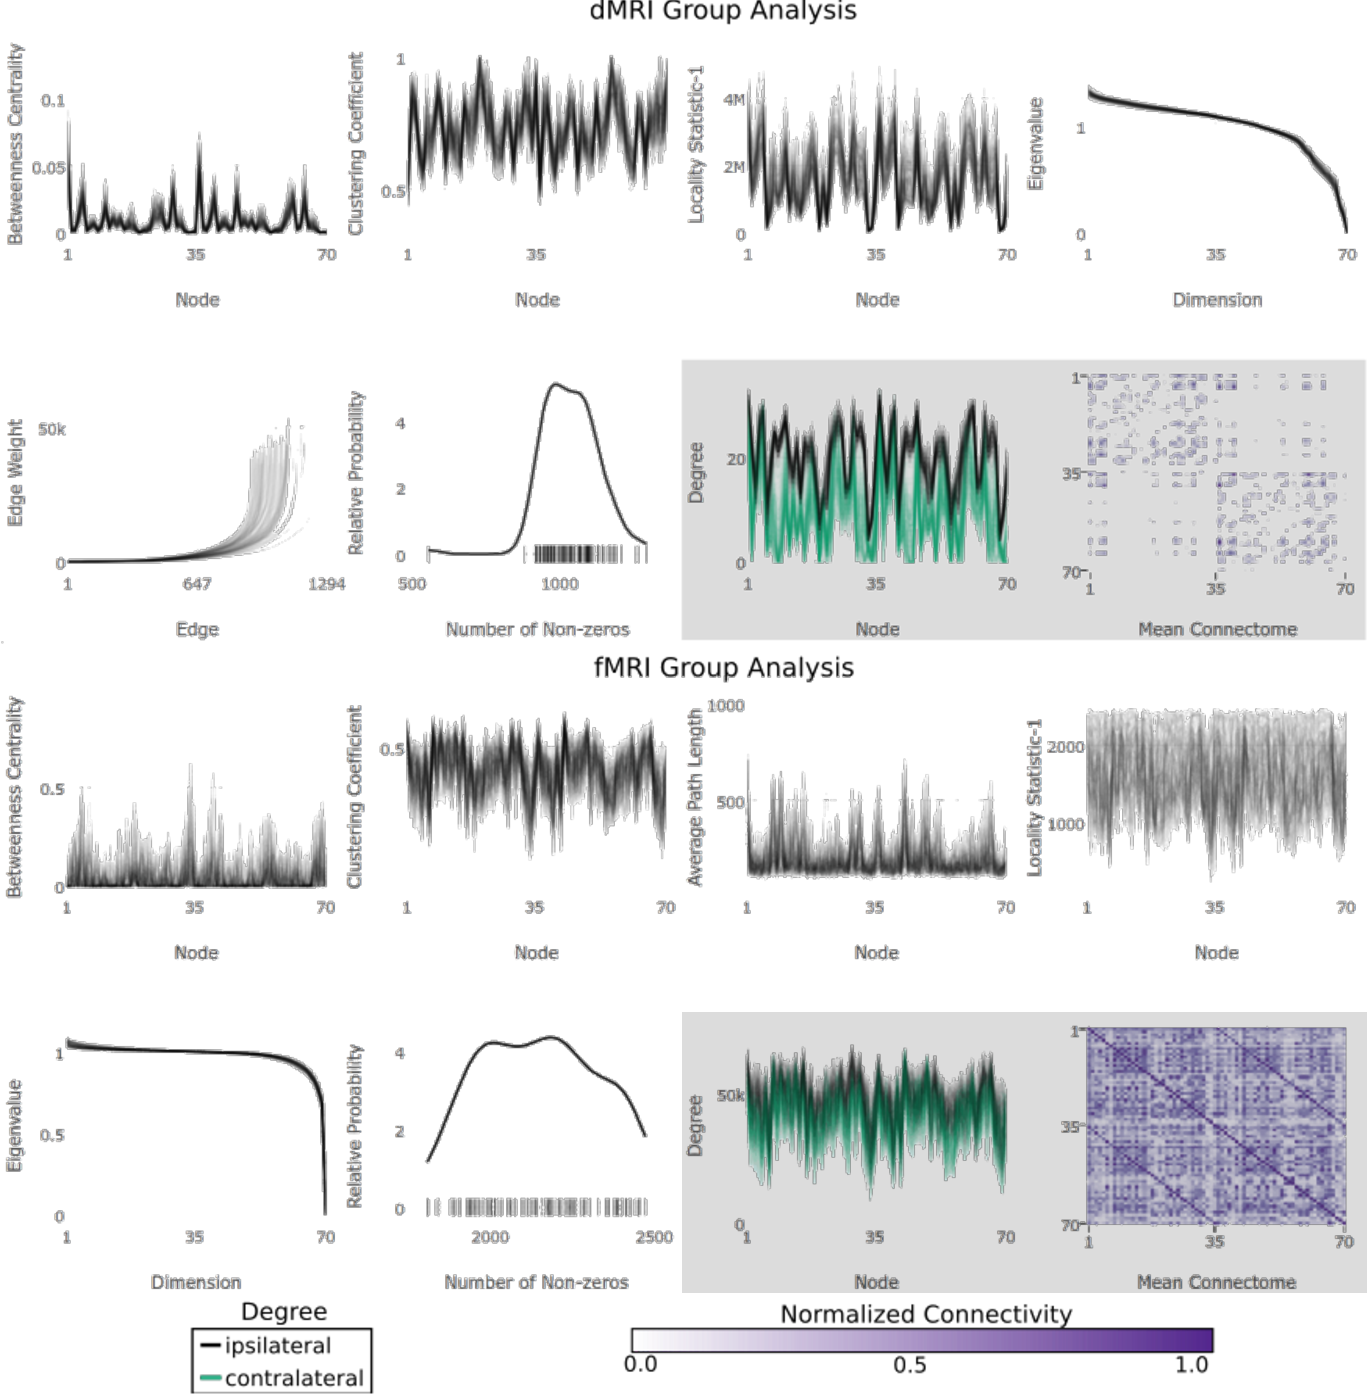
\includegraphics[width=\textwidth]{./figs/fig_graphqa.pdf}
\caption{\textbf{\ndmg's group level analysis computes and plots eight connectome-specific summary statistics per modality for each scan, providing immediate quality assurance for the entire study.} In theory, any connectome could be an outlier for any of these statistics, so plotting all of them together is particularly useful (see~\ref{app:graphstats} for details). The top panels  show results for the BNU1 dMRI connectomes, the bottom panels show the results for the BNU1 fMRI connectomes.
}
\label{fig:graphqa}
\end{figure*}
%%%%%%%

% \paragraph{Group Level Implementation Strategy}

Leveraging previous efforts developed in our  ``Science in the Cloud''~\cite{sic} manuscript, multiple scans and studies are evaluated in parallel for participant-level analysis, and the derivatives are pooled for group-level analysis, much like typical map-reduce approaches (consistent with the BIDS app specification~\cite{bidsapps}). The parallel  implementation uses the Amazon Web Services (AWS) cloud, in particular leveraging their storage (S3) and high performance computing (Batch) services. Data are stored in an S3 bucket enabling  the \ndmg~cloud-API connectome estimation pipeline to process all scans on Amazon Batch in parallel. In practice,  AWS limits the number of parallel threads users are allowed to launch (to prevent accidental spending). After connectome estimation is complete, the same cloud-API exposed by \ndmg~enables group-level analysis to be launched and parallelized across each parcellation for all scans within each study. We were able to compute diffusion connectomes at 24~scales for each of the publicly available 2,861~scans (totaling 68,664~connectomes) in under one day and \$1,000. Had we processed each scan in parallel, cost would have remained the same but only taken $1.5$~hours.

% \paragraph{Group-Level Graph Summary Statistics}

Each scan's estimated connectome can be summarized by a set of graph statistics, as described above. For group-level analysis, we visualize each scan's summary statistics overlaid on one another. For example, Figure~\ref{fig:graphqa} demonstrates that each diffusion graph from the BNU3 dataset using the Desikan atlas has relatively similar values for the statistics (we use the Desikan atlas for the remainder of the analyses unless otherwise specified). Moreover, it is clear from both the degree plot and the mean connectome plot that the dMRI connectomes from this study tend to have more connections within a hemisphere than across a hemisphere, as expected. For the fMRI connectomes, however, the homotopic connections---that is, connections from one region on a hemisphere to the same region on the other hemisphere---seem particularly strong.
%Supplementary Figure ~\ref{fig:graphqaf} shows example group-level analysis for the same study's functional data.
 
%\ref{app:multi} illustrates how \ndmg~also computes the average value for each univariate and multivariate statistic for each atlas, and demonstrates similarities across scales, indicating that that the basic structure of the connectomes is preserved across different atlases.


%\subsubsection{\ndmgf~Individual-Level Pipeline}

\subsection{Group-Level Multi-Scale Analysis}

For both diffusion and functional MRI, the QA for graph generation includes a heat map of the adjacency matrix, the number of non-zero edges, and several multivariate graph statistics (one statistic per vertex in the graph) including:  betweenness centrality, clustering coefficient, hemisphere-separated degree sequence, edge weight, eigenvalues of the graph laplacian, and locality statistic-1~\cite{glocal}.
We developed the hemisphere-separated degree sequence to indicate the ipsilateral and contralateral degree for each vertex, which we found quite useful for QA.  
\ref{app:graphgenf} includes definitions and implementation details for each of the statistics.
Supplementary Figure ~\ref{fig:multiscale} shows, for a single individual, the graph summary statistics for the multi-connectome (including both functional and diffusion) across the set of atlases described above.


%%%%%%%
% \begin{table*}
    \centering
    \caption{\textbf{\ndmg~pipeline robustness and reliability.}
We ran \ndmg~on over 20 different studies, including both fMRI and dMRI data, spanning multiple different scanners, acquisition parameters, and population demographics. Nonetheless, for both fMRI and dMRI data, across all datasets with multiple measurements, \ndmg~always achieved $>0.8$ discriminability, and \ndmgd's discriminability was typically $>0.98$ on the dMRI data. MM computes discriminability using multi-modal data from both the dMRI and fMRI connectomes. $D$=discriminability. Scanners are G (GE), P (Phillips), or S (Siemens).	
}
    \label{tab:data}
    \pgfplotstabletypeset[
    	header=true,
        string type,
        font=\addfontfeature{Numbers={Monospaced}}\small,
        columns/dset/.style={column name=Study, column type={p{.115\textwidth}}},
        columns/sca/.style={column name=Scanner, column type={p{.06\textwidth}}},
        columns/age/.style={column name={Age$\pm$1 std}, column type={p{.106\textwidth}}},
        columns/male/.style={column name=$\%$ Male, column type={p{.06\textwidth}}},
        columns/subjs/.style={column name=Indiv., column type={p{.055\textwidth}}},
        columns/ses/.style={column name=Ses., column type={p{.04\textwidth}}},
        columns/totd/.style={column name=\#Scans, column type={p{.049\textwidth}}},
        columns/trtd/.style={column name=$D$, column type={p{.048\textwidth}}},
        columns/totf/.style={column name=\#Scans, column type={p{.049\textwidth}}},
        columns/trtf/.style={column name=$D$, column type={p{.048\textwidth}}},
        columns/totm/.style={column name=\#Scans, column type={p{.049\textwidth}}},
        columns/trtm/.style={column name=$D$, column type={p{.048\textwidth}}},
        every head row/.style={
            before row={
            	\topline
                \rowcolor{tableheadcolor}
                & & & & & &\multicolumn{2}{c}{dMRI} & \multicolumn{2}{c}{fMRI} & \multicolumn{2}{c}{MM} \\
                \rowcolor{tableheadcolor}
            },
            after row={\midtopline}
        },
        every odd row/.style={
        	before row={\rowcolor{vlgray}}
        },
        every row no 25/.style={
            before row={\topline\rowcolor{tableheadcolor}}
        },
        every last row/.style={
            before row={\rowcolor{tableheadcolor}},
            after row=\bottomline
        },  
        col sep=&,
        row sep=\\
    ]{dset & sca & age & male & subjs & ses & totd & trtd & totf & trtf & totm & trtm \\
    HNU1~\cite{corr} & G & 24.4 $\pm$ 2.3 & 0.50 & 30  & 10 & 300 & 0.993 & 300 & 0.956 & 300 & .993 \\
    BNU1~\cite{corr} & S & 23.0 $\pm$ 2.3 & 0.53 & 57  & 2  & 114 & 0.984 & 108 & 0.906 & 108 & .990 \\
    SWU4~\cite{corr} & S & 20.0 $\pm$ 1.3 & 0.51 & 235 & 2 & 454 & 0.884 & 466 & 0.891 & 452 & .903 \\
    BNU3~\cite{corr} & S & 22.5 $\pm$ 2.1 & 0.50 & 48 & 1 & 47 & NA & 47 & NA  & 47 & NA \\
    Kirby21~\cite{Kirby21}  & P  & 31.8 $\pm$ 9.4 & 0.52 & 21 & 2 & 42 & 1.0 & -- & -- & -- & -- \\
    NKI1~\cite{corr} & S & 34.4 $\pm$ 12.8 & 0.0 & 24 & 2 & 40 & 0.984 & -- & --& -- & -- \\
    Temp114 & S & 21.8 $\pm$ 3.0 & 0.58 & 114 & 1 & 114 & NA & -- & --& -- & -- \\
    NKI-ENH~\cite{nkirs} & S & 42.5 $\pm$ 19.6 & 0.40 & 198 & 1 & 198 & NA & -- & --& -- & -- \\
    Temp255 & S & 22.1 $\pm$ 3.9 & 0.51 & 255 & 1 & 253 & NA & -- & --& -- & -- \\
    PING~\cite{ping} & G/S/P & 11.7 $\pm$ 5.0 & 0.52 & 932 & 1-5 & 1486 & NA &-- &  --& -- & -- \\
    MRN1313 & S  & 27.6 $\pm$ 13.3 & 0.60 & 1313 & 1 & 1299 & NA &-- &  -- & --  & --\\
    IPCAS6~\cite{corr} & S & 23.0 $\pm$ 2.0 & 0.5 & 2 & 9 & -- & -- & 18 & 0.994& -- & -- \\
    IPCAS8~\cite{corr} & S & 57.6 $\pm$ 3.6 & 0.46 & 13 & 2 & -- & -- & 26 & 0.958 & --  & -- \\
    SWU1~\cite{corr} & S & 21.6 $\pm$ 1.7 & 0.3 & 20 & 3 & -- & -- & 60 & 0.935 & --  & -- \\
    IPCAS5~\cite{corr} & S & 18.3 $\pm$ 0.5 & 1.0 & 22 & 2 & -- & -- & 44 & 0.819 & --  & --\\
    SWU3~\cite{corr} & S & 20.4 $\pm$ 1.6 & .35 & 23 & 2 & -- & -- & 46 & 0.986 & -- & -- \\
    XHCUMS~\cite{corr} & S & 52.0 $\pm$ 6.3 & 0.60 & 23 & 5 & -- & -- & 115 & 0.823 & -- & --\\
    UWM~\cite{corr} & G & 25.0 $\pm$ 3.2 & 0.56 & 25 & 2 & -- & -- & 50 & 0.849 & -- & -- \\
    NYU1~\cite{corr} & S & 29.4 $\pm$ 8.4 & 0.4 & 25 & 3 & -- & -- & 75 & 0.931 & -- & -- \\
    SWU2~\cite{corr} & S & 21.0 $\pm$ 1.6 & 0.33 & 27 & 2 & -- & -- & 54 & 0.874 & -- & --\\
    IPCAS1~\cite{corr} & S & 20.9 $\pm$ 1.7 & 0.3 & 30 & 2 & -- & -- & 60 & 0.893 & -- & --\\
    IPCAS2~\cite{corr} & S & 13.4 $\pm$ 0.9 & 0.35 & 34 & 2 & -- & -- & 68 & 0.868 & -- & --\\
    IBATRT~\cite{corr} & S & 28.0 $\pm$ 7.5 & 0.54 & 36 & 2 & -- & -- & 50 & 0.974 & -- & --\\
    MRN1~\cite{corr} & S & 15.1 $\pm$ 7.8 & 0.5 & 52 & 2 & & & 90 & 0.859 & -- & --\\
    BNU2~\cite{corr} & S & 20.9 $\pm$ .9 & 0.54 & 61 & 2 & -- & -- & 121 & 0.863 & -- & --\\
    Pooled dMRI & & & & 3227 & & 4347 & 0.979 & -- & -- & -- & --\\
    Pooled fMRI & & & & 763 & &  -- & -- & 1798 & 0.881 & -- & --\\
    Pooled MM & & & & 361 & & -- & -- & -- & -- & 907 & 0.982 \\
    }
\end{table*}
%%%%%%%


%%%%%%%
\begin{figure*}[b!]
\centering
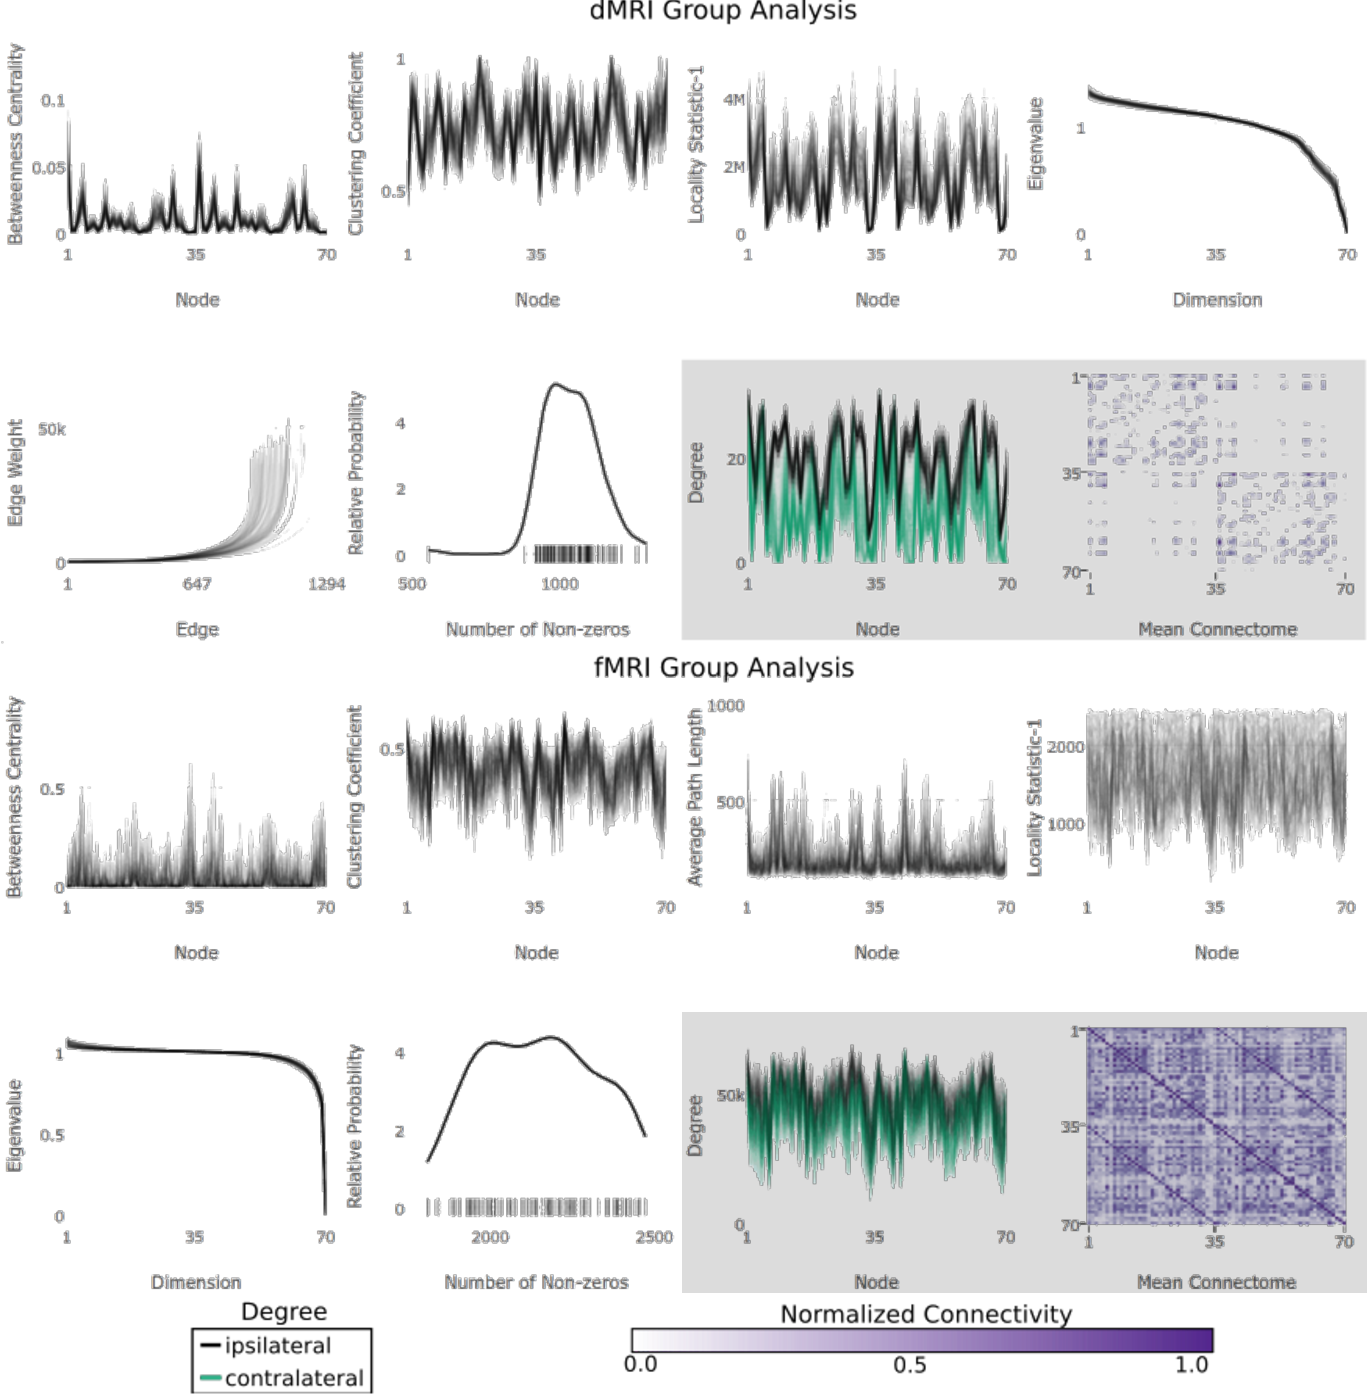
\includegraphics[width=\textwidth]{./figs/fig_graphqa.pdf}
\caption{\textbf{\ndmg's group level analysis computes and plots eight connectome-specific summary statistics per modality for each scan, providing immediate quality assurance for the entire study.} In theory, any connectome could be an outlier for any of these statistics, so plotting all of them together is particularly useful (see~\ref{app:graphstats} for details). The top panels  show results for the BNU1 dMRI connectomes, the bottom panels show the results for the BNU1 fMRI connectomes.
}
\label{fig:graphqa}
\end{figure*}
%%%%%%%

% \paragraph{Group Level Implementation Strategy}

Leveraging previous efforts developed in our  ``Science in the Cloud''~\cite{sic} manuscript, multiple scans and studies are evaluated in parallel for participant-level analysis, and the derivatives are pooled for group-level analysis, much like typical map-reduce approaches (consistent with the BIDS app specification~\cite{bidsapps}). The parallel  implementation uses the Amazon Web Services (AWS) cloud, in particular leveraging their storage (S3) and high performance computing (Batch) services. Data are stored in an S3 bucket enabling  the \ndmg~cloud-API connectome estimation pipeline to process all scans on Amazon Batch in parallel. In practice,  AWS limits the number of parallel threads users are allowed to launch (to prevent accidental spending). After connectome estimation is complete, the same cloud-API exposed by \ndmg~enables group-level analysis to be launched and parallelized across each parcellation for all scans within each study. We were able to compute diffusion connectomes at 24~scales for each of the publicly available 2,861~scans (totaling 68,664~connectomes) in under one day and \$1,000. Had we processed each scan in parallel, cost would have remained the same but only taken $1.5$~hours.

% \paragraph{Group-Level Graph Summary Statistics}

Each scan's estimated connectome can be summarized by a set of graph statistics, as described above. For group-level analysis, we visualize each scan's summary statistics overlaid on one another. For example, Figure~\ref{fig:graphqa} demonstrates that each diffusion graph from the BNU3 dataset using the Desikan atlas has relatively similar values for the statistics (we use the Desikan atlas for the remainder of the analyses unless otherwise specified). Moreover, it is clear from both the degree plot and the mean connectome plot that the dMRI connectomes from this study tend to have more connections within a hemisphere than across a hemisphere, as expected. For the fMRI connectomes, however, the homotopic connections---that is, connections from one region on a hemisphere to the same region on the other hemisphere---seem particularly strong.
%Supplementary Figure ~\ref{fig:graphqaf} shows example group-level analysis for the same study's functional data.
 
%\ref{app:multi} illustrates how \ndmg~also computes the average value for each univariate and multivariate statistic for each atlas, and demonstrates similarities across scales, indicating that that the basic structure of the connectomes is preserved across different atlases.


\subsection{Group-Level Multi-Scale Analysis}
\label{app:multi}

Figure~\ref{fig:multiscale} top panel shows the group-level summary statistics of diffusion connectomes belonging to same dataset over 13 parcellations ranging from 48 nodes up to 500 nodes; for clarity, an additional 11 parcellations with up to over 70,000 nodes are not shown here. The bottom panel shows the group-level summary statistics of functional connectomes belonging to the same dataset over 5 parcellations ranging from 52 to 200 nodes. 
For each parcellation, vertex statistics are normalized by dividing them into number of vertices in the parcellation, and then smoothed via kernel-density estimation to enable comparison across scales. The kernel-width was computed using Scott's Rule, the default mode for Scipy (\url{https://docs.scipy.org/doc/scipy-0.19.1/reference/generated/scipy.stats.gaussian_kde.html}).
For most of the statistics, the ``shape'' of the distributions  are relatively similar across scales, though their actual magnitudes can vary somewhat dramatically.
%In particular, in Figure~\ref{fig:multiscale}, graphs from the the downsampled block-atlases (DS) appear to be scaled versions of one another, as may be expected because they are related to one-another by a region-growing function~\cite{glocal}.

%%%%%%%
\begin{figure*}[b!]
\centering
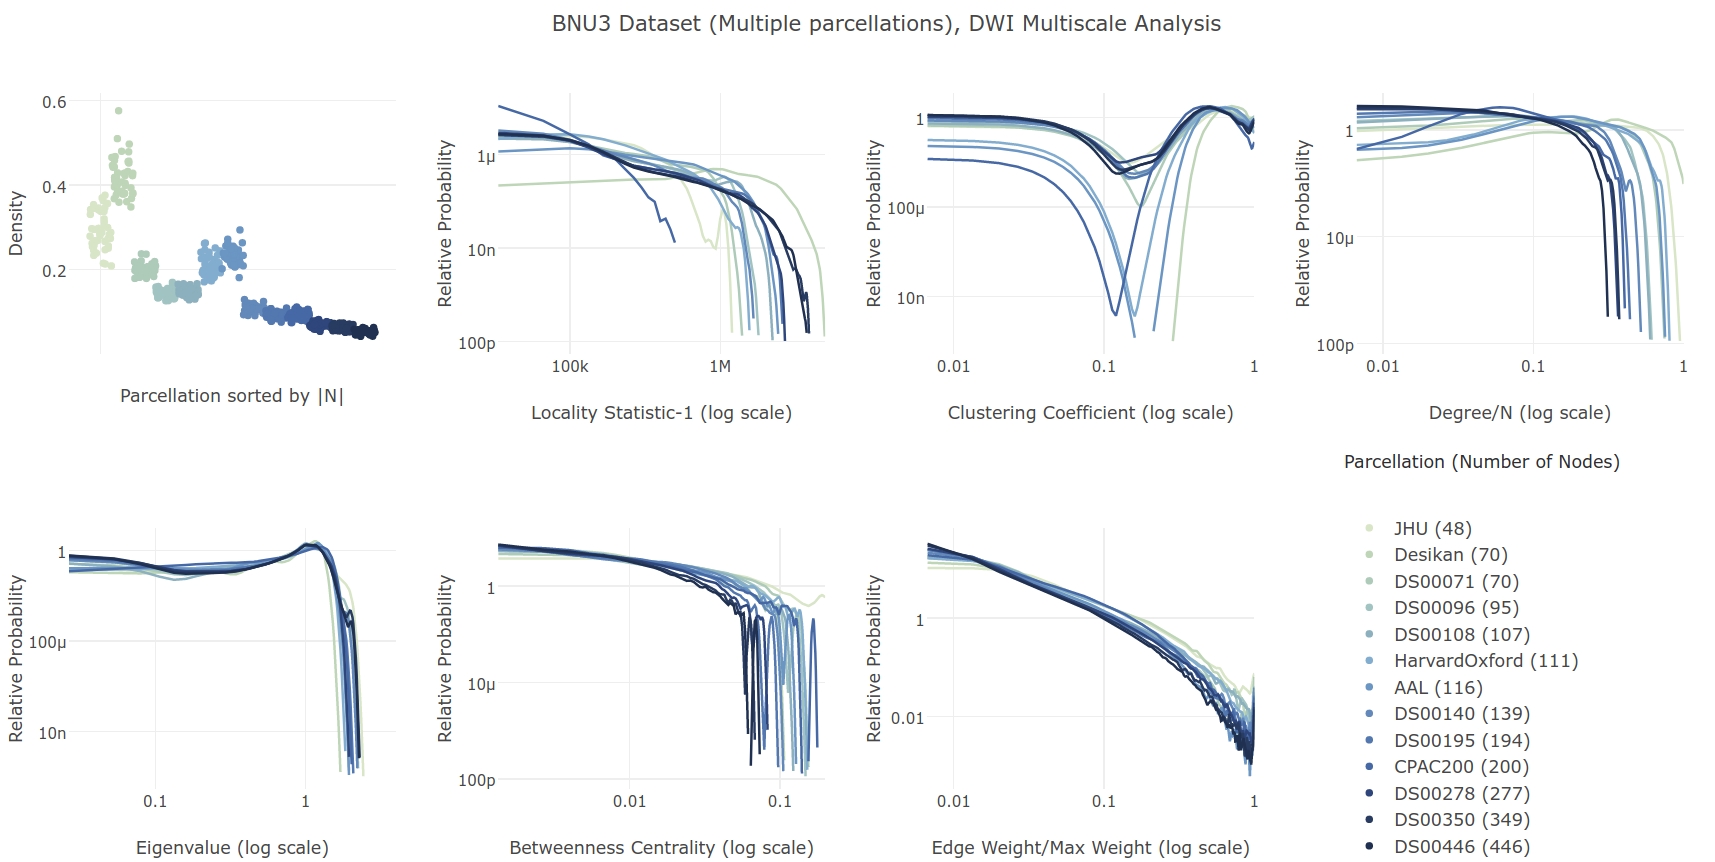
\includegraphics[width=\textwidth]{./figs/fig_multiscale.png}
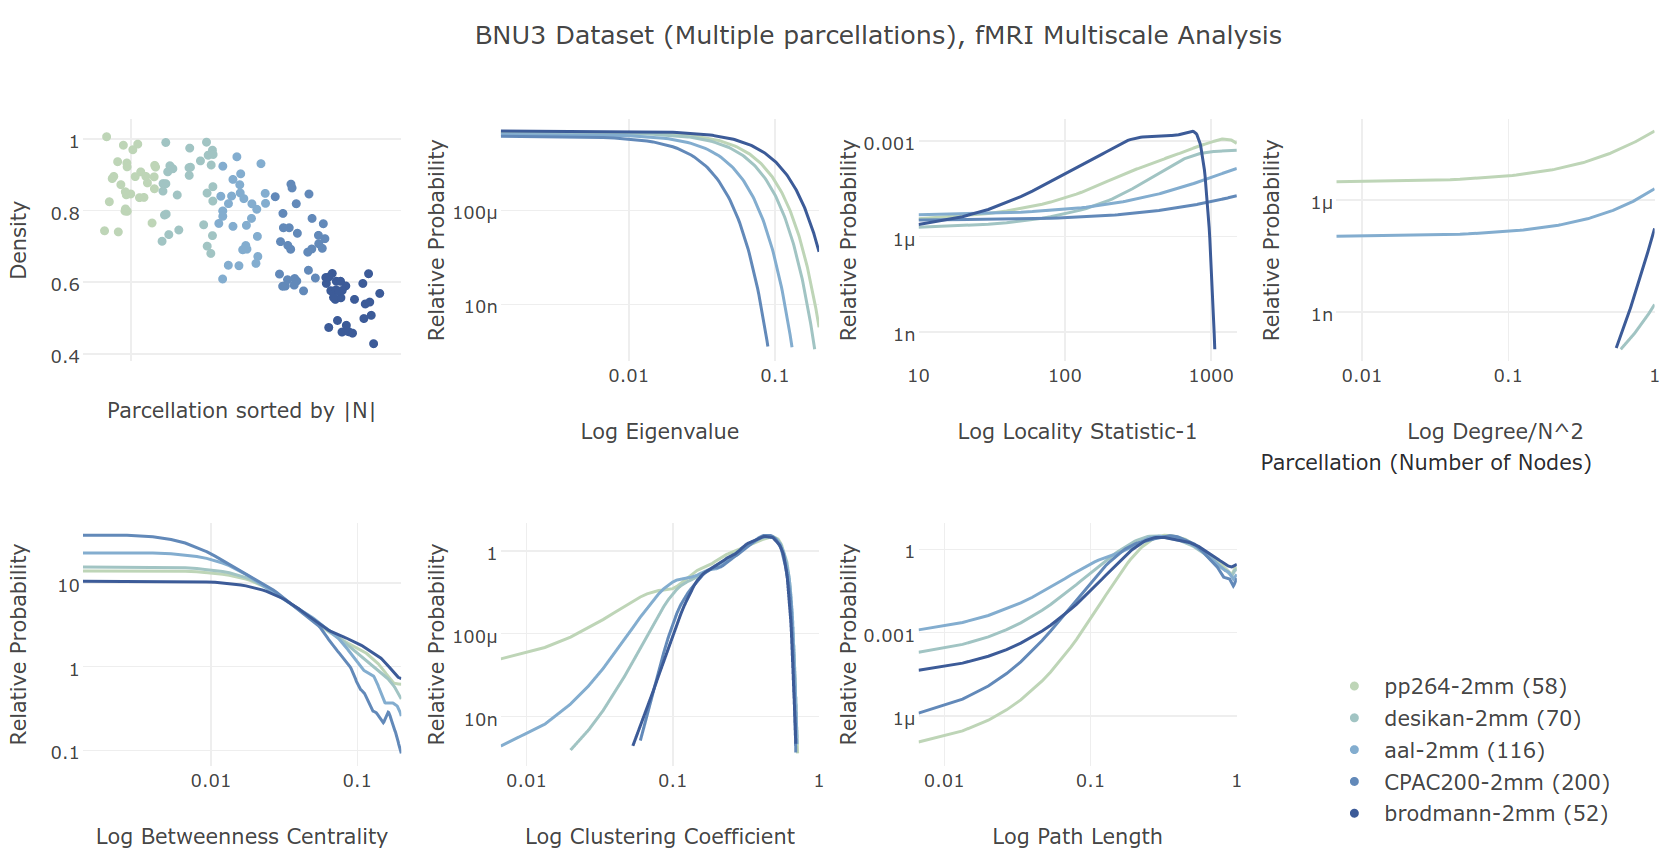
\includegraphics[width=\textwidth]{./figs/fig_fmri_multiscale.png}
\caption{\textbf{Multi-Scale Connectome Analysis.}
\ndmg~produces connectomes at a variety of scales, enabling investigation
of graph properties between parcellation schemes. We can observe that the statistics are qualitatively similar in shape
across scales, however, they are quantitatively significantly different, for both the diffusion (top) and functional (bottom) connectomes. This suggests that claims made or analyses
performed on a given scale may not hold when applied to another scale. This is impactful, as the choice of parcellation
has significant bearing on the results of a scientific study.}
% @gk: why don't we have ipsi-lateral and contra-lateral broken out here?
% @gk: i don't understand from the text what the curves are.  are they averages over subjects within this group? if so, specify.
\label{fig:multiscale}
\end{figure*}
%%%%%%%



%\clearpage


\section{Availability Statements}

\subsection{Code Availability}

All of our code is available from our website, \url{http://m2g.io/},  and has been deposited into our public github repository, \url{https://github.com/neurodata/ndmg}, and published with a DOI, \url{https://doi.org/10.5281/zenodo.1161284}, under the Apache License 2.0. 

\subsection{Data Availability}

The data derivatives that support the findings of this study are available from our website, \url{http://m2g.io/},  under a (ODC-By) v1.0 license.


\end{document}
